% Generated from article/index.html by article_to_tex.py; edit the HTML snapshot for content changes.
FEE $\rightarrow$ Sampler $\rightarrow$ STFBuilder $\rightarrow$ TimeFrameBuilder $\rightarrow$ LogicFilter $\rightarrow$ TimeFrameSlicerByLogicTiming $\rightarrow$ FilterTimeFrameBySomething $\rightarrow$ FileSink。各段階のデータを、既存のKeynote図と同じ色分けの入れ子図で示す。図中の並びは上から下がデータ順。箱の面積はbyte数に比例しない。\textbf{太字は前段から追加・変更された要素}を示す。


\FloatBarrier
\subsection{対象と読み方}
この資料はnestdaq-user-implのローカルスナップショットをもとに、v1ヘッダとV3 TDCを中心に整理したものです。対象コードの内容は行番号付きの参照ソース、SHA-256はソースmanifestに記録しています。NestDAQ全運用・全世代を一律に規定するものではありません。

緑：TF、橙：STF、灰青：HBF、濃灰：DAQ word/HBD、青緑：Filter/Trigger、濃い緑：同期したheartbeat group、ウォームグレー：FileSink。\textit{S}＝TFのソース数、\textit{H}＝1ソースのSTFに含むHBF数、\textit{n\textsubscript{j}}＝HBF jのtrigger数。概念上の枠の見出しは左揃え、実際に記録されるHeader・DAQ words・HBD・TrgTimeは中央揃え。DAQ wordsの下にHBDを別の箱で示す。代表例では複数の要素を描き、「$\times$ number of …」は図示分を含む総繰り返し数を表す。


\FloatBarrier
\subsection{デバイスを通るデータ構造}
\label{sec:format-html-pipeline}

\subsubsection{max-hbfが決めるパッキングの単位}
\textbf{Heartbeat groupは、時刻同期された同じHeartbeatを共通の基準とする、複数ソース（FEM）のDAQ wordのまとまり}を表す。各ソースの同じheartbeat区間を対応付け、そのHBD情報をMETA、同じ区間内のtrigger窓で切り出したDAQ wordをSLICEとしてまとめる。単に受信順が近いデータを束ねたものではない。

\texttt{STFBuilder --max-hbf H} $\rightarrow$ 各ソースのSTFにH個のHBF $\rightarrow$ 元のTF区間にH個のheartbeat位置 $\rightarrow$ Slicerが\textbf{H個のMETAレコード}を生成。各METAに、そのHBFで見つかったtrigger数だけSLICEレコードが続く。


\FloatBarrier
{\footnotesize\setlength{\tabcolsep}{3pt}\begin{longtable}{p{0.24\linewidth}p{0.66\linewidth}}
\caption{max-hbfが決めるパッキングの単位。}\label{tab:format-html-1}\\
\hline
段階 & 1つの元TF区間に対応する構造 \\ \hline\endfirsthead
\hline 段階 & 1つの元TF区間に対応する構造 \\ \hline\endhead
{STFBuilder} & {各FEM：STF Header + HBF $\times$ \textit{H}。\textit{H} = \texttt{max-hbf}} \\
{TimeFrameBuilder} & {TF Header + STF $\times$ ソース数。各STFは同じ\textit{H}個のheartbeat位置を持つ} \\
{Slicer} & {[META\textsubscript{j} + SLICE $\times$ \textit{n\textsubscript{j}}] $\times$ \textit{H}個のheartbeat group} \\
{後段Filter} & {[META\textsubscript{j} + 採用SLICE $\times$ \textit{k\textsubscript{j}}] $\times$ \textit{H}。0 $\leq$ \textit{k\textsubscript{j}} $\leq$ \textit{n\textsubscript{j}}} \\
\hline\end{longtable}}
例：\texttt{max-hbf=3}、各HBFのtrigger数が2、0、1なら、出力順は \texttt{[META$_0$, SLICE$_0$,$_0$, SLICE$_0$,$_1$] [META$_1$] [META$_2$, SLICE$_2$,$_0$]}。METAは3個、SLICEの合計は3個。triggerが0個のHBFにもMETAは残る。

Slicer以後の図では、これらを共通の\textbf{TimeFrame（元の入力TF区間）}の外枠で囲み、その中へHBFごとのまとまりを入れる。外枠とheartbeat groupは説明用の概念で、追加のHeaderやlengthを持つ保存レコードではない。実際のTF Header(type=META/SLICE)は各レコードの先頭にあり、METAとSLICEはbyte列上で順に並ぶ。

上の個数関係は各ソースのHBFが揃う通常の入力を想定する。\texttt{max-hbf}の既定値は1、1未満の指定は1へ補正される（パラメータ読出し、既定値）。Slicerはmax-hbfのオプション値を直接読むのではなく、入力中の実HBF数に沿って反復する（実HBF数）。


\subsubsection{FEE}
FEE出力の連続word列。HBDを含み、ソフトウェアのHBF Headerはまだない。

図のDAQ wordを1 wordずつ描き、複数ヒットの区間と0ヒットの区間を並べた。半透明・破線のDAQ wordは任意／不在を示す説明用の印であり、その位置に空のwordが記録される意味ではない。0ヒットでもHBD1/HBD2は区間の末尾に現れる。

FEE（Front-End Electronics）がヒットのTDC・TOT・CH番号などをDAQ wordとして出力し、heartbeat区間の末尾にHBD1/HBD2を挿入する。図では通常のhitとHBDを示す。実際にはthrottlingやspillなどの制御wordもあり、任意の64 bit wordをhitとして読むことはできない。

元のメモにある周期は524.288 $\mu$s。HBDの周期はハードウェア・firmware側の仕様として扱い、今回のソフトウェアコードだけから周期設定を確定してはいない。時刻を説明する際は「HBDに対応するheartbeat区間内の相対時刻」と、STFのUNIX時刻を分ける。


図\ref{fig:format-svg-01-fee}に示す。
\begin{figure}[htbp]\centering
\makebox[\linewidth][c]{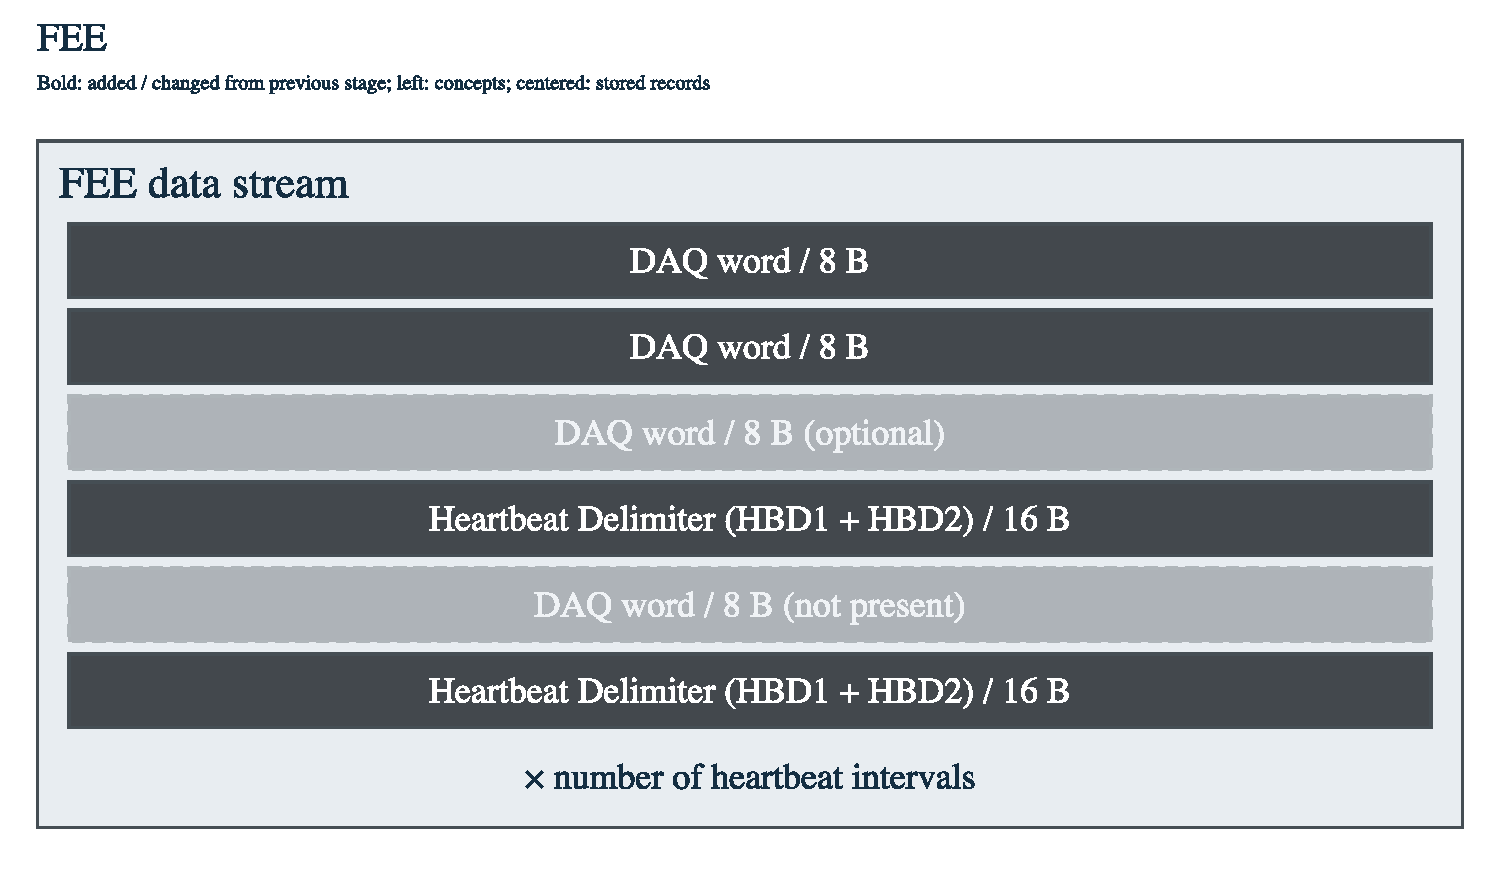
\includegraphics[pagebox=cropbox,width=0.95\linewidth,height=0.70\textheight,keepaspectratio]{../figure/10-3-nestdaq-dataformat/pdf/01-fee.pdf}}
\caption{FEEの出力。DAQ wordは0個以上。先頭の区間は複数hitの例、続く区間は0 hitの例。各区間はHBDで終わる。半透明・破線のwordは任意／不在の説明用で、空wordが記録されるわけではない。}\label{fig:format-svg-01-fee}\end{figure}

\subsubsection{Sampler}
コードでは受信したword列をFairMQ messageへ入れて送信。元資料の参考図2のHBFラップは実装上STFBuilderで行う。FEMInfoは別の初期化メッセージ。

実機用の \texttt{AmQStrTdcSampler} は、受信バッファをそのままサイズ付きのFairMQ messageに載せて送る（受信データの送信処理）。受信chunkの境界はHBD境界と一致するとは限らない。後段のSTFBuilderは残りのwordを保持して次の受信と結合する。

初期化時には別途24 byteのFEMInfoを送れる（SendFEMInfo）。magicは \texttt{0x4f464e492d4d4546}、LE文字列は \texttt{"FEM-INFO"}。送信処理ではoffset 8にFEMType、12にFEMIdを配置し、16〜23はreserved。C++構造体宣言のFEMId/FEMTypeの順序とは違うため、受信wire配置は送信処理で確認する。

参考の2.pngはHBF Header付きの姿を示す。今回の実装ではそのHeaderを付けるのはSTFBuilderなので、この段階の図はコードに合わせて受信word列とした。HBFという論理区間と、HBF Headerを付けた出力オブジェクトを区別する。


図\ref{fig:format-svg-02-sampler}に示す。
\begin{figure}[htbp]\centering
\makebox[\linewidth][c]{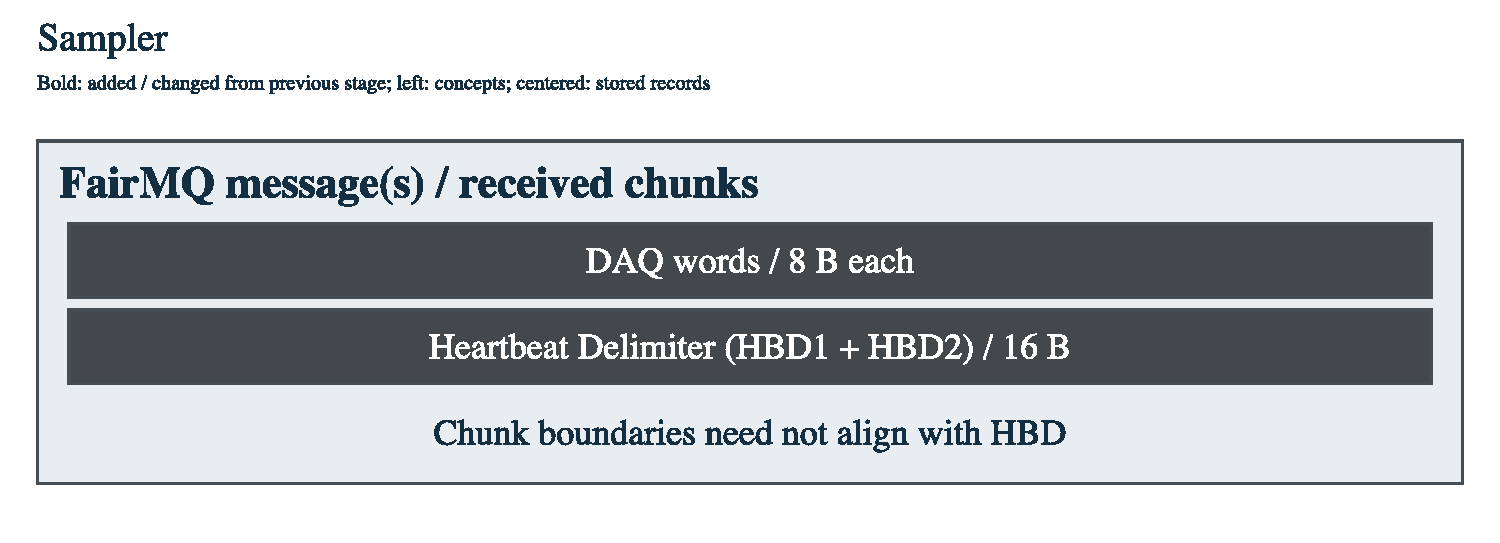
\includegraphics[pagebox=cropbox,width=0.95\linewidth,height=0.70\textheight,keepaspectratio]{../figure/10-3-nestdaq-dataformat/pdf/02-sampler.pdf}}
\caption{Samplerの出力。}\label{fig:format-svg-02-sampler}\end{figure}

\subsubsection{STFBuilder}
STFBuilderのmax-hbfで、STFあたりにまとめるHBF数を指定する。通常の揃った入力ではH = max-hbf。

HBDを認識し、受信chunkをまたぐデータも集めて、HBF Header 16 byteを追加する（FillData）。末尾のHBDもpayloadとして残る。HBFの \texttt{length} はHeaderとpayloadの合計。

\texttt{max-hbf}で指定したHBF数に達するとSTF Header 48 byteを先頭に置く。ソースのFEM種別・ID、timeFrameId、タイムスタンプを設定する（FinalizeSTF）。STFの \texttt{length} はHeaderを含む全メッセージ長の合計、\texttt{numMessages} はSTF Headerを除くpayloadメッセージ数。この経路では各payloadがHBFなので、ここではHBF数に対応する。

FairMQ multipartの概形は \texttt{[STF Header] [HBF 0] [HBF 1] …}。HBF HeaderとDAQ word/HBDは同じpartに格納される。


図\ref{fig:format-svg-03-stfbuilder}に示す。
\begin{figure}[htbp]\centering
\makebox[\linewidth][c]{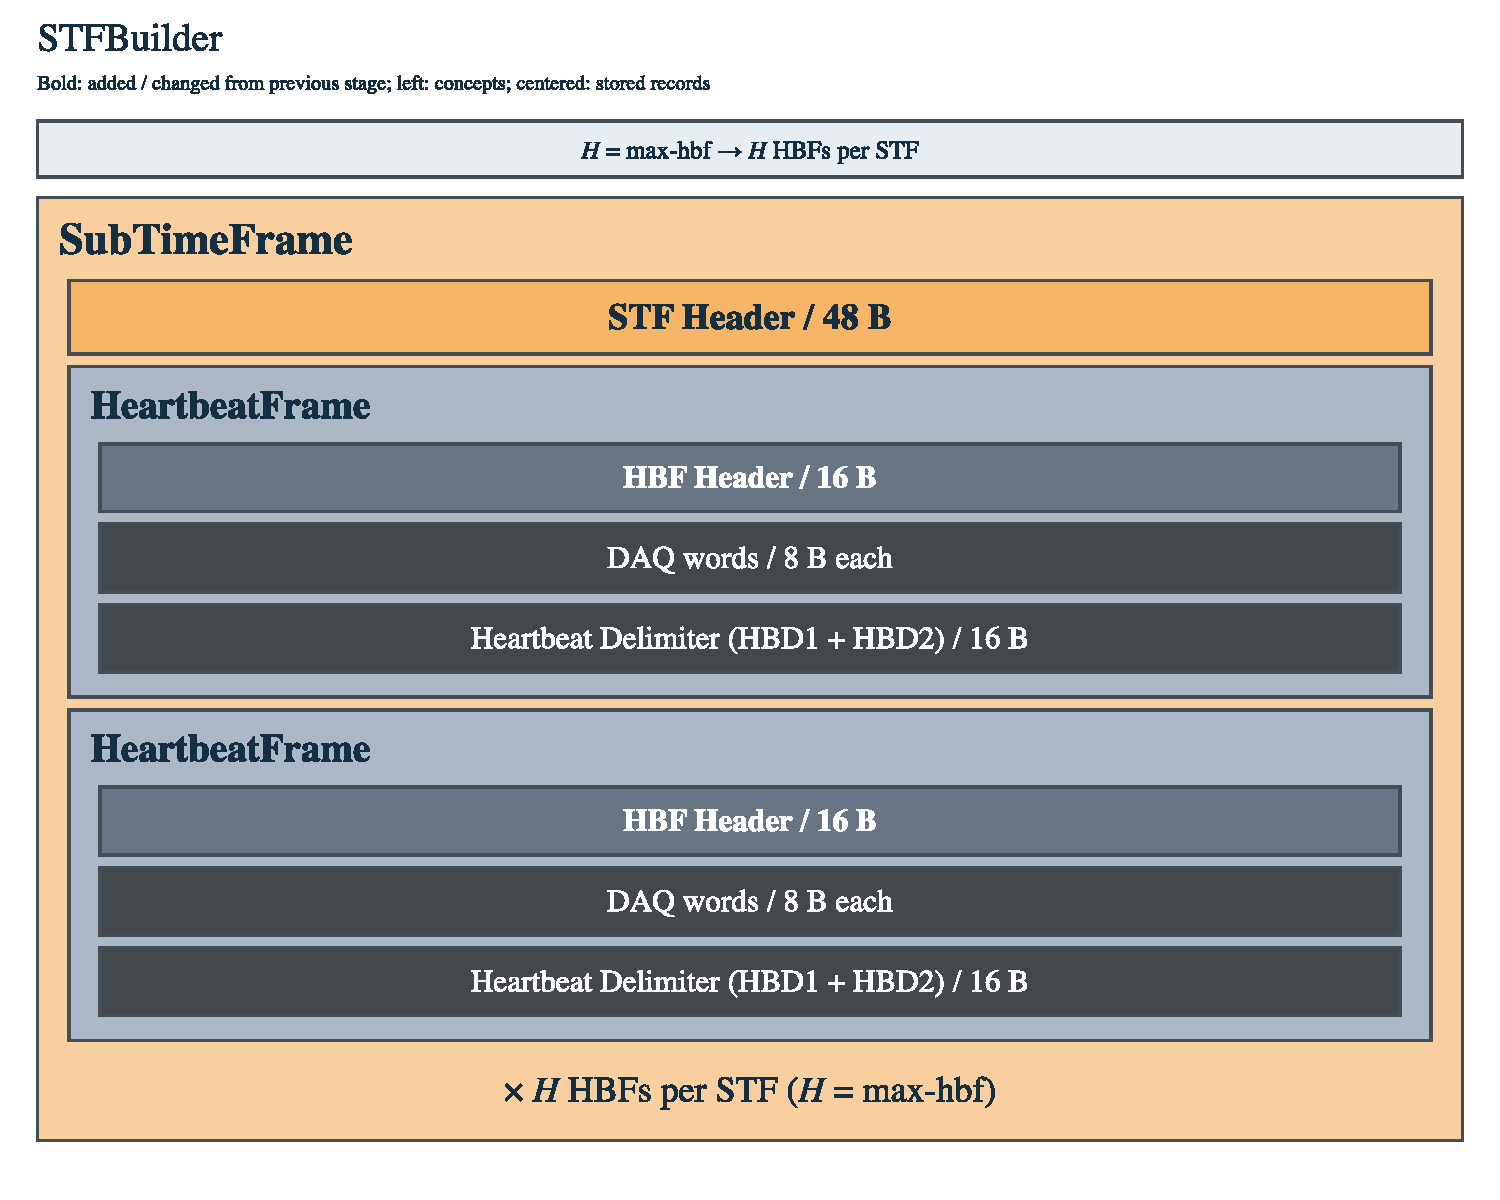
\includegraphics[pagebox=cropbox,width=0.95\linewidth,height=0.70\textheight,keepaspectratio]{../figure/10-3-nestdaq-dataformat/pdf/03-stfbuilder.pdf}}
\caption{STFBuilderの出力。}\label{fig:format-svg-03-stfbuilder}\end{figure}

\subsubsection{TimeFrameBuilder}
同じtimeFrameIdのSTFをソース間で集約。TF Headerの後に各ソースのSTFが並ぶ。

各FEMからのSTFをtimeFrameIdで対応付け、必要なソースが揃ったTFを構築する。単に異なる時刻のSTFを足し合わせるのではなく、同じIDに属するソースの集合をまとめる。ソース数Sは通常の構成では読み出しFEM数に対応するが、実際には設定と参加ソースの集合で決まる。

出力は \texttt{[TF Header] [source 0のSTF Header] [そのHBF列] [source 1のSTF Header] [そのHBF列] …}。Headerは24 byteで、numSource、timeFrameId、全長を設定する（TFの生成処理）。既存STFのメッセージを出力multipartへ移すため、DAQ wordのbit配置はここでは変わらない。


図\ref{fig:format-svg-04-timeframebuilder}に示す。
\begin{figure}[htbp]\centering
\makebox[\linewidth][c]{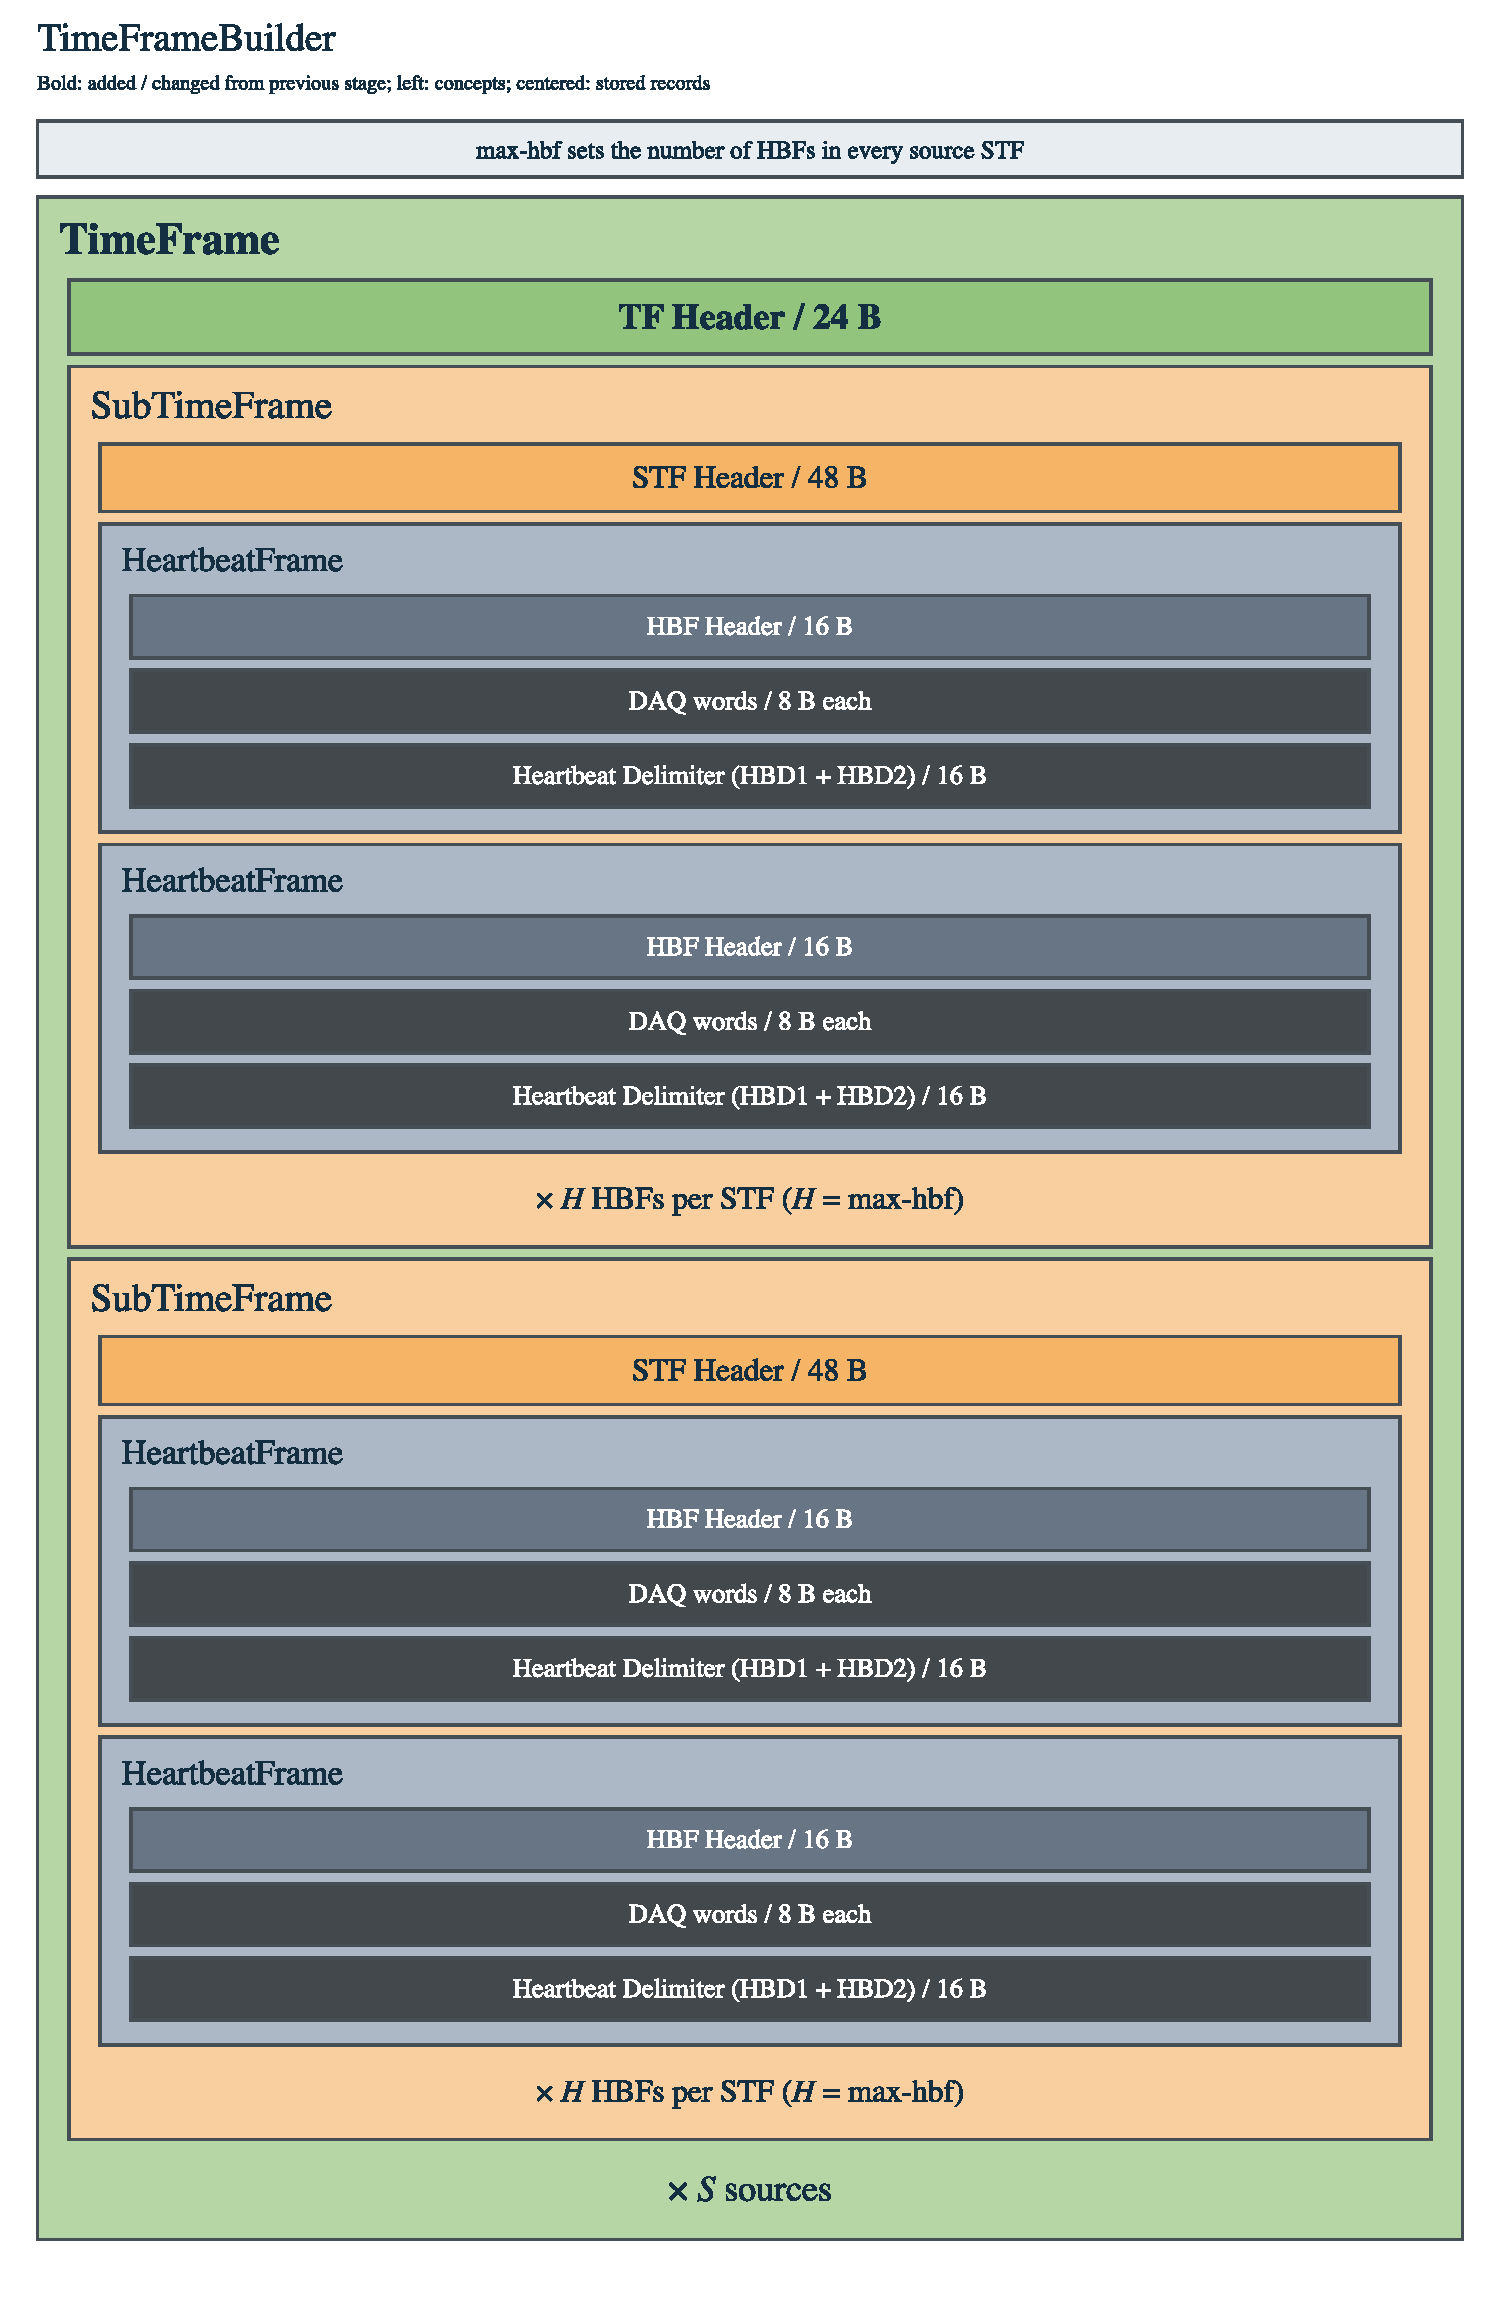
\includegraphics[pagebox=cropbox,width=0.95\linewidth,height=0.70\textheight,keepaspectratio]{../figure/10-3-nestdaq-dataformat/pdf/04-timeframebuilder.pdf}}
\caption{TimeFrameBuilderの出力。}\label{fig:format-svg-04-timeframebuilder}\end{figure}

\subsubsection{LogicFilter}
単一のFilter HeaderとHBF別のTrigger TimeブロックをTF HeaderとSTF列の間へ挿入。

各HBF内のヒットをソース間で照合し、設定した論理条件の成立時刻を求める。TF Headerの直後に、\textbf{単一のFilter Header}と、HBFごとの \texttt{[Trigger Time Header][TrgTime列]} を追加する。その後にSTF列が続く（出力の組み立て、Filter情報の生成）。参考5.pngにはFilter Headerが複数描かれているが、この実装経路では1個。

Trigger Time Headerは16 byte、TrgTimeは1個8 byte。\texttt{numTrigs = $\sum$ n\_\allowbreak{}j}、\texttt{Filter::\allowbreak{}numMessages = 1 + H}。各HBFのtriggerが0個でも、そのHBFに対応するTrigger Time Headerを持ち得る。TrgTimeは \texttt{uint32\_\allowbreak{}t time} と \texttt{uint32\_\allowbreak{}t type} の組で、LogicFilterはtypeに \texttt{0xaa000000} を書く。

data suppressionを有効にした経路では、送らないHBFのDAQ wordを落とし、Headerと末尾HBD2 wordを持つblank HBFに置き換える場合がある（BlankHBF）。図はtrigger情報の追加が見える代表構造。DAQ wordが常に全量保存されるとは限らない。


図\ref{fig:format-svg-05-logicfilter}に示す。
\begin{figure}[htbp]\centering
\makebox[\linewidth][c]{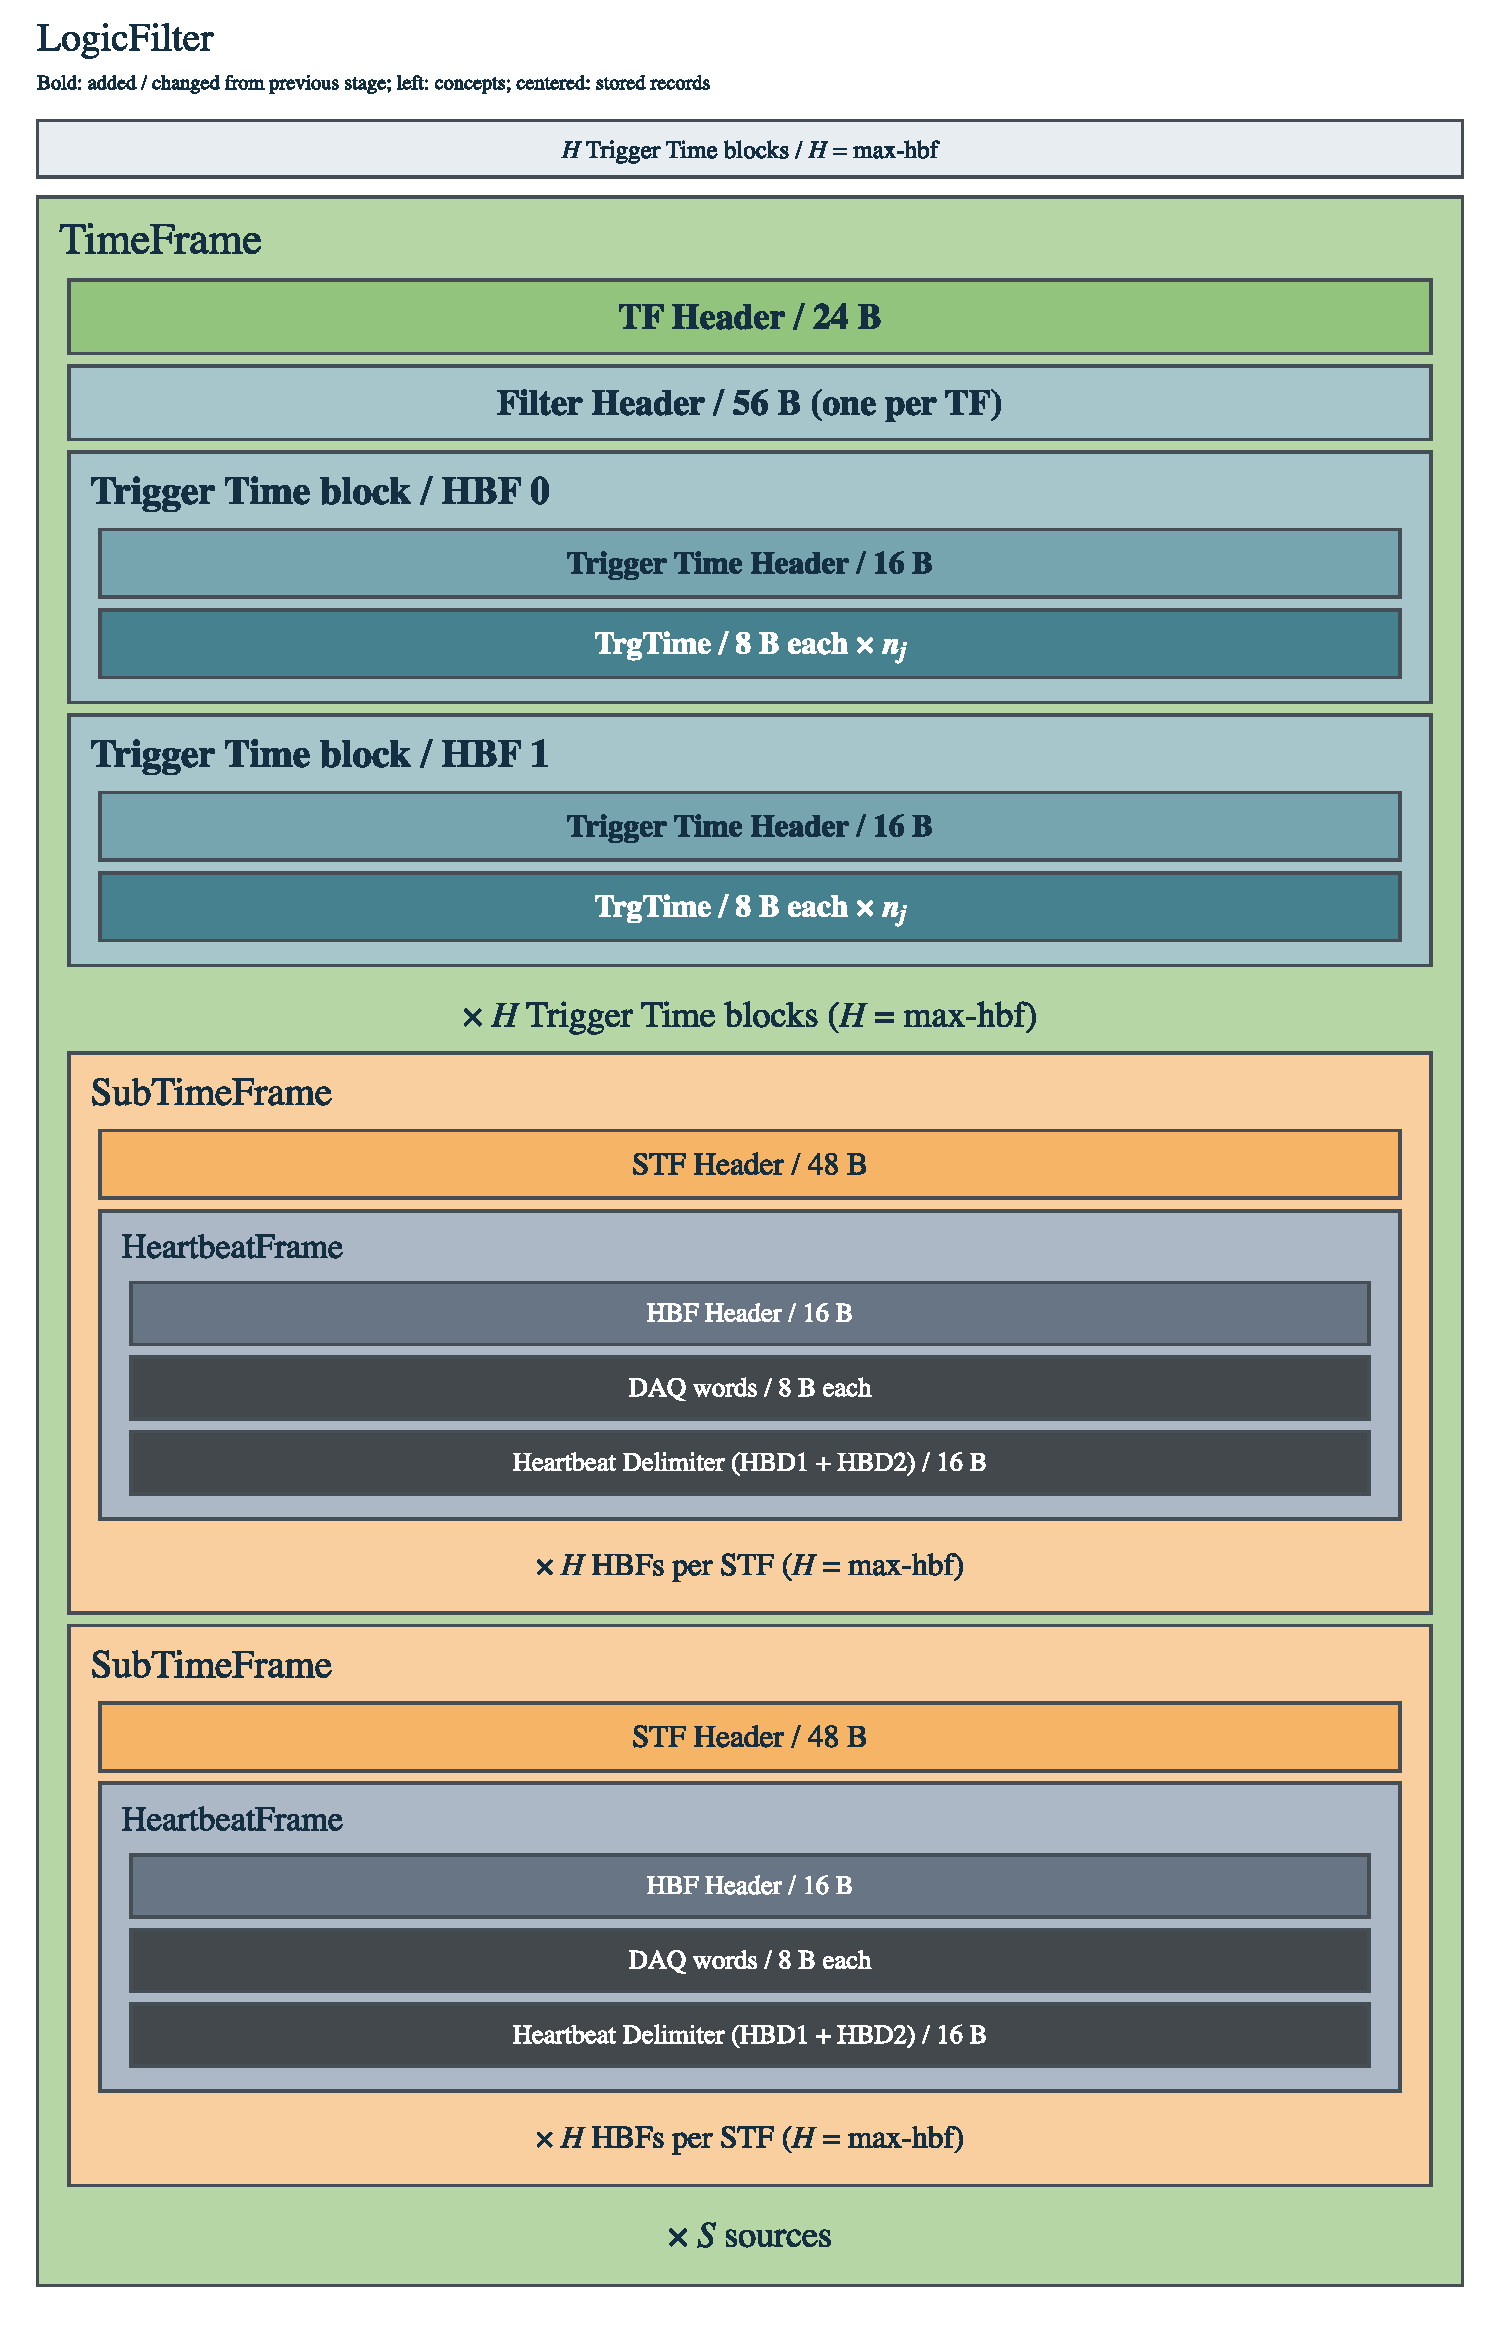
\includegraphics[pagebox=cropbox,width=0.95\linewidth,height=0.70\textheight,keepaspectratio]{../figure/10-3-nestdaq-dataformat/pdf/05-logicfilter.pdf}}
\caption{LogicFilterの出力。}\label{fig:format-svg-05-logicfilter}\end{figure}

\subsubsection{TimeFrameSlicerByLogicTiming}
HBF jごとにMETA TFを1個、そのHBFの各triggerにつきSLICE TFを1個生成。METAにHBDとtrigger情報、SLICEに窓内DAQ wordとHBDを収める。

入力TFのHBF番号jに注目し、\texttt{[META TF\_\allowbreak{}j] [SLICE TF\_\allowbreak{}j,0] … [SLICE TF\_\allowbreak{}j,n\_\allowbreak{}j−1]} を作る。これを各HBFについて繰り返す。入力1 TFから、基本形では \textbf{H個のMETA TFと$\sum$n\_j個のSLICE TF} が生まれる（HBFごとの反復）。実装のfNumHBFは最後にパースしたSTFのHBF数から決まる。欠損・不揃い入力は別途確認が必要。

\textbf{META：}TF HeaderのtypeをMETAにし、Filter Header・HBF jのTrigger Time HeaderとTrgTime列、各ソースのSTF Header・HBF Header・HBDを入れる。通常のデータSTFではDAQ wordをコピーせず、末尾のHBD2 wordだけを残す。入力STFが既にMETAの場合はそのHBFデータ全体をコピーする例外がある（METAの作成）。

\textbf{SLICE：}triggerごとにTF HeaderのtypeをSLICEにし、各データソースから \texttt{trig + offsetBegin $\leq$ tdc4n $\leq$ trig + offsetEnd} のDAQ wordを取り出す。HBFの末尾HBD2 wordもコピーする。META型の入力STFはSLICEには含めない。Trigger情報そのものはSLICE内には入らず、直前のMETA側に置かれる（triggerごとのSLICE作成）。

各HBFの \texttt{META + SLICE列} は1個の連続バッファ／FairMQ partにシリアライズされる。図では元の入力区間をTimeFrameの共通外枠で囲む。その中のMETA/SLICEは順に並ぶ独立レコードであり、外枠の分だけ追加Headerが付くわけではない。窓が重なるtriggerについては読み出し位置を戻すため、同じhitが複数SLICEに含まれることもある。


図\ref{fig:format-svg-06-slicer}に示す。
\begin{figure}[htbp]\centering
\makebox[\linewidth][c]{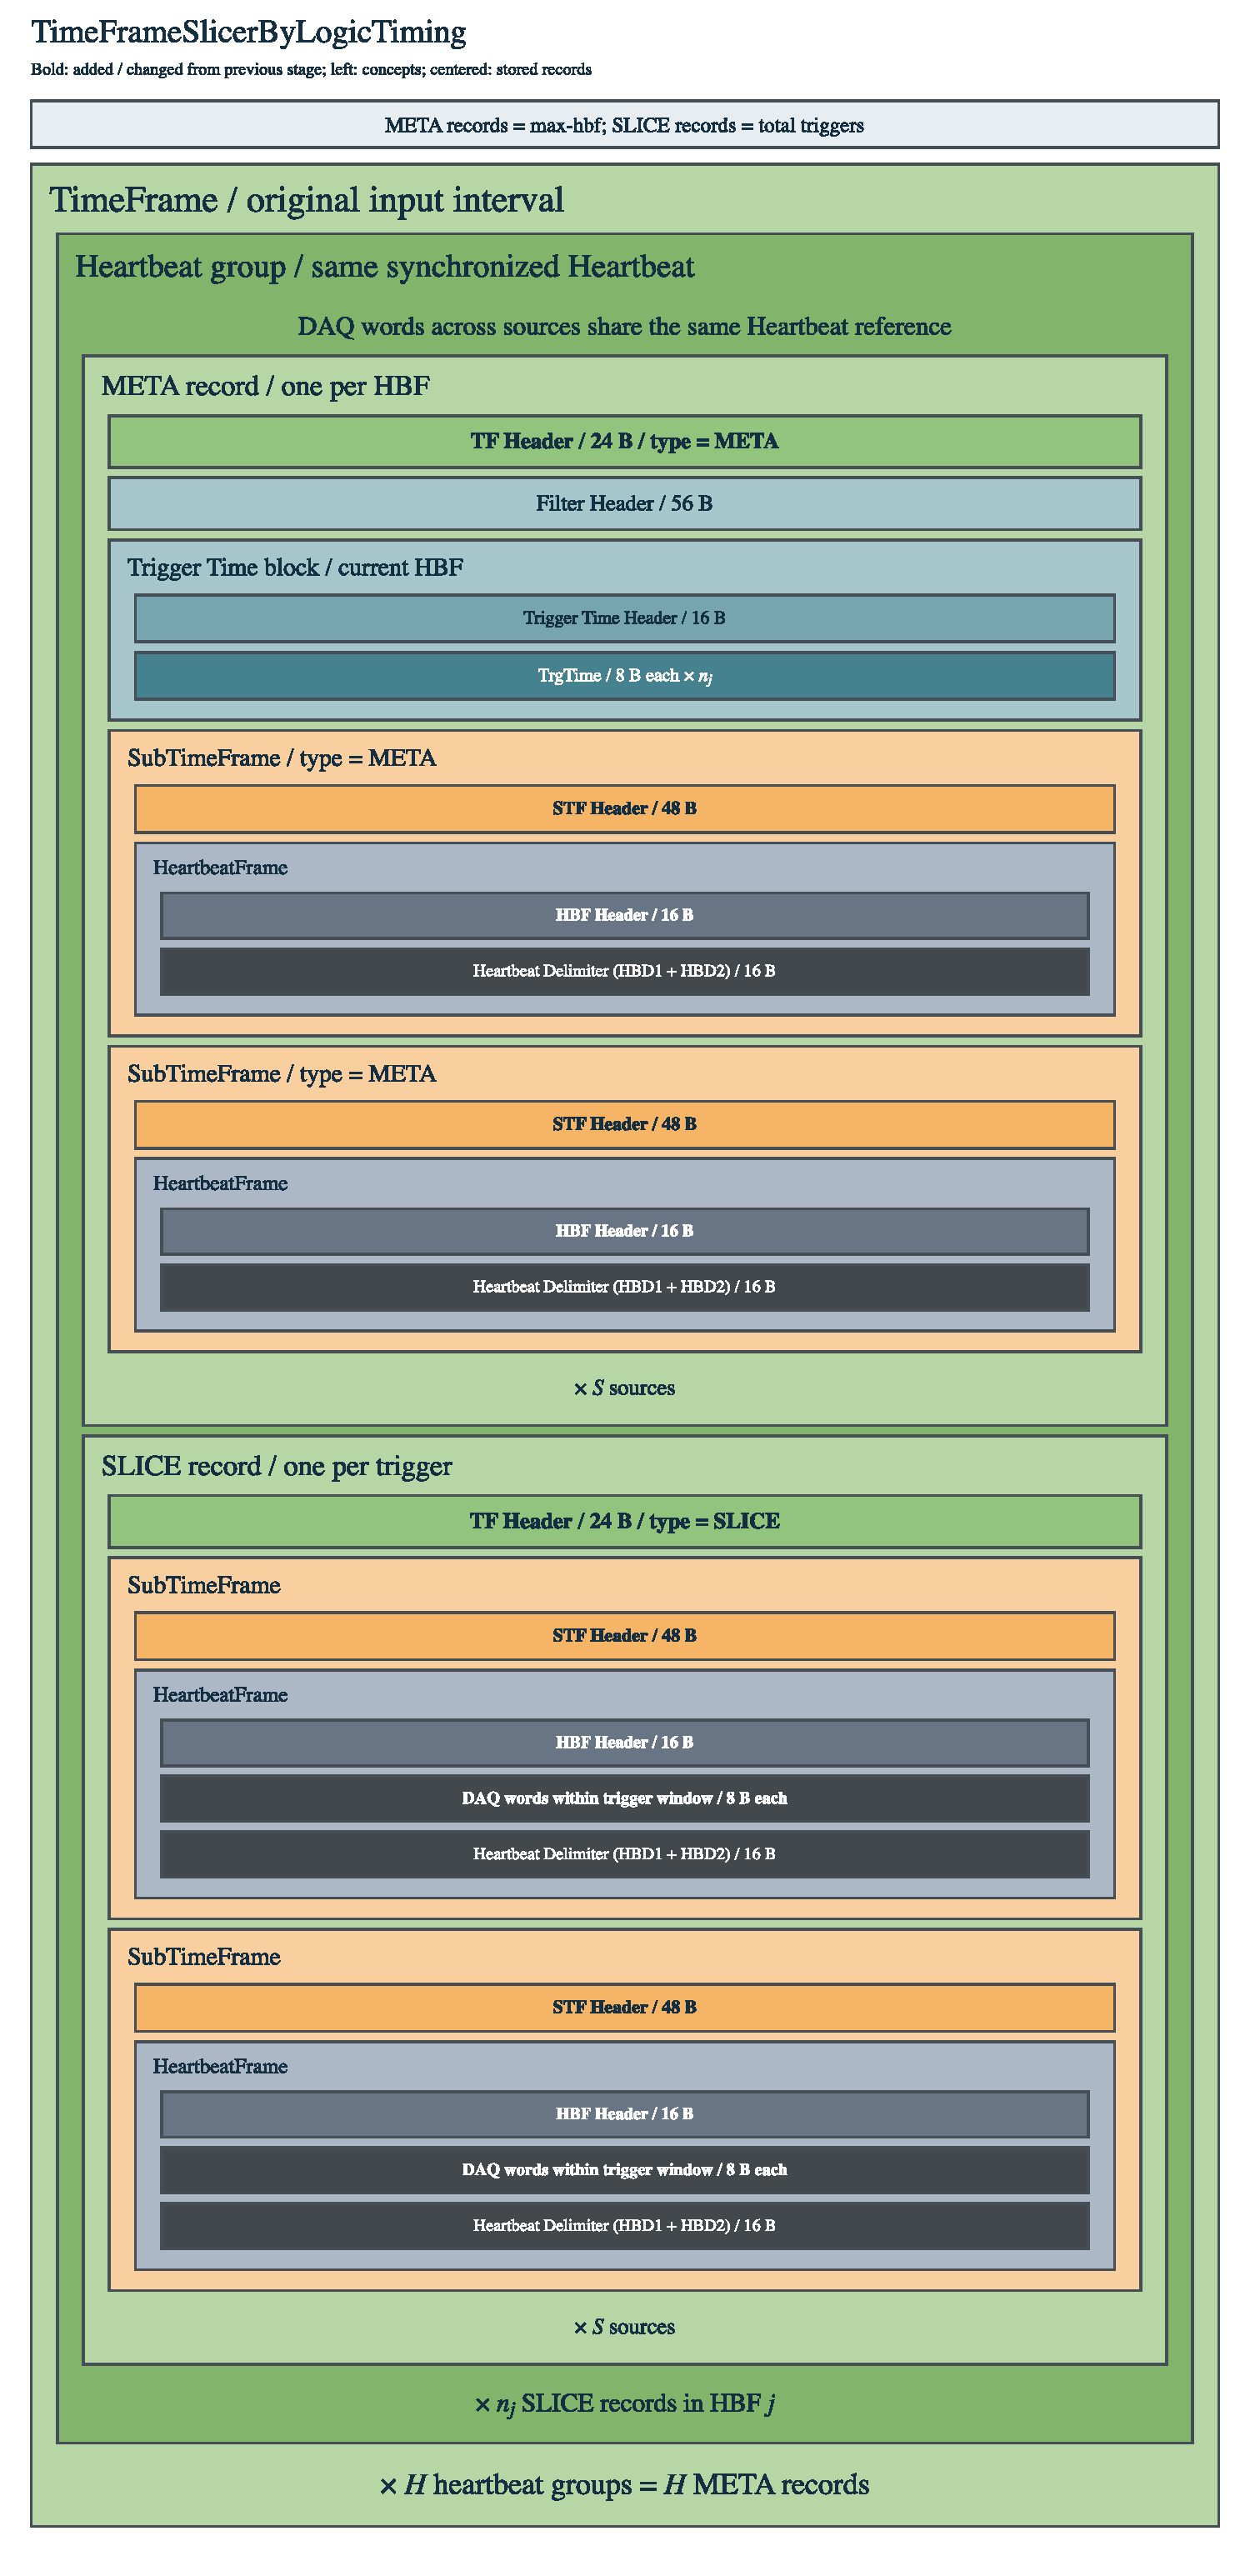
\includegraphics[pagebox=cropbox,width=0.95\linewidth,height=0.70\textheight,keepaspectratio]{../figure/10-3-nestdaq-dataformat/pdf/06-slicer.pdf}}
\caption{TimeFrameSlicerByLogicTimingの出力。}\label{fig:format-svg-06-slicer}\end{figure}

\subsubsection{FilterTimeFrameSlice / high level filter}
実装名はFilterTimeFrameSliceBySomething。METAを保持、SLICEはProcessSliceで選択。Filter/Trigger Time情報は再シリアライズ時に落ちる。現状のBySomethingは全SLICEを保持。

ここでの実ファイル名は \texttt{FilterTimeFrameSliceBySomething}。共通の \texttt{FilterTimeFrameSliceABC::\allowbreak{}ParseMessages} が、連続バッファからTF/STF/HBFを \texttt{FrameContainer.h} のコンテナへパースする。Filter Headerは読み飛ばし、Trigger Timeブロックはlengthぶん進めるため、再出力用のコンテナには含めない（ParseMessages）。

共通処理はMETAを無条件に保持し、その他のTFは \texttt{ProcessSlice(tf)} の結果で保持する。採用されたTFを \texttt{CopyAllTo} で再出力するため、METAのFilter/Trigger情報はこの段階で除かれる。TFのlengthは再計算される（選別と再出力、コンテナのシリアライズ）。

BySomethingはhigh level filterのスケルトンであり、現在の有効なProcessSlice()は \texttt{return true;} なので、SLICEはすべて残る（雛形の実装）。7.pngの「SLICEを落とす」表現は、具体的な選別処理を実装した場合の動作。TOT・TOF・Multiplicity等の派生フィルタで選別条件を与える。左右の比較図はこの選別動作の例であり、現在のスケルトンがSLICEを落とすことを示すものではない。ただしMETAのFilter/Trigger情報を除く共通処理は、ProcessSlice()のreturn trueとは独立して行われる。

\textbf{選別動作の例：}左は入力、右は不採用SLICEを半透明・破線で示した説明図。不採用SLICEとFilter/Trigger情報は実際の出力byte列には存在しない。表示位置を揃えて消えた部分を比較するために描いている。現在のBySomethingのProcessSlice()はreturn trueなので、このSLICE除去はまだ行わない。


図\ref{fig:format-svg-07-filter-input}に示す。
\begin{figure}[htbp]\centering
\makebox[\linewidth][c]{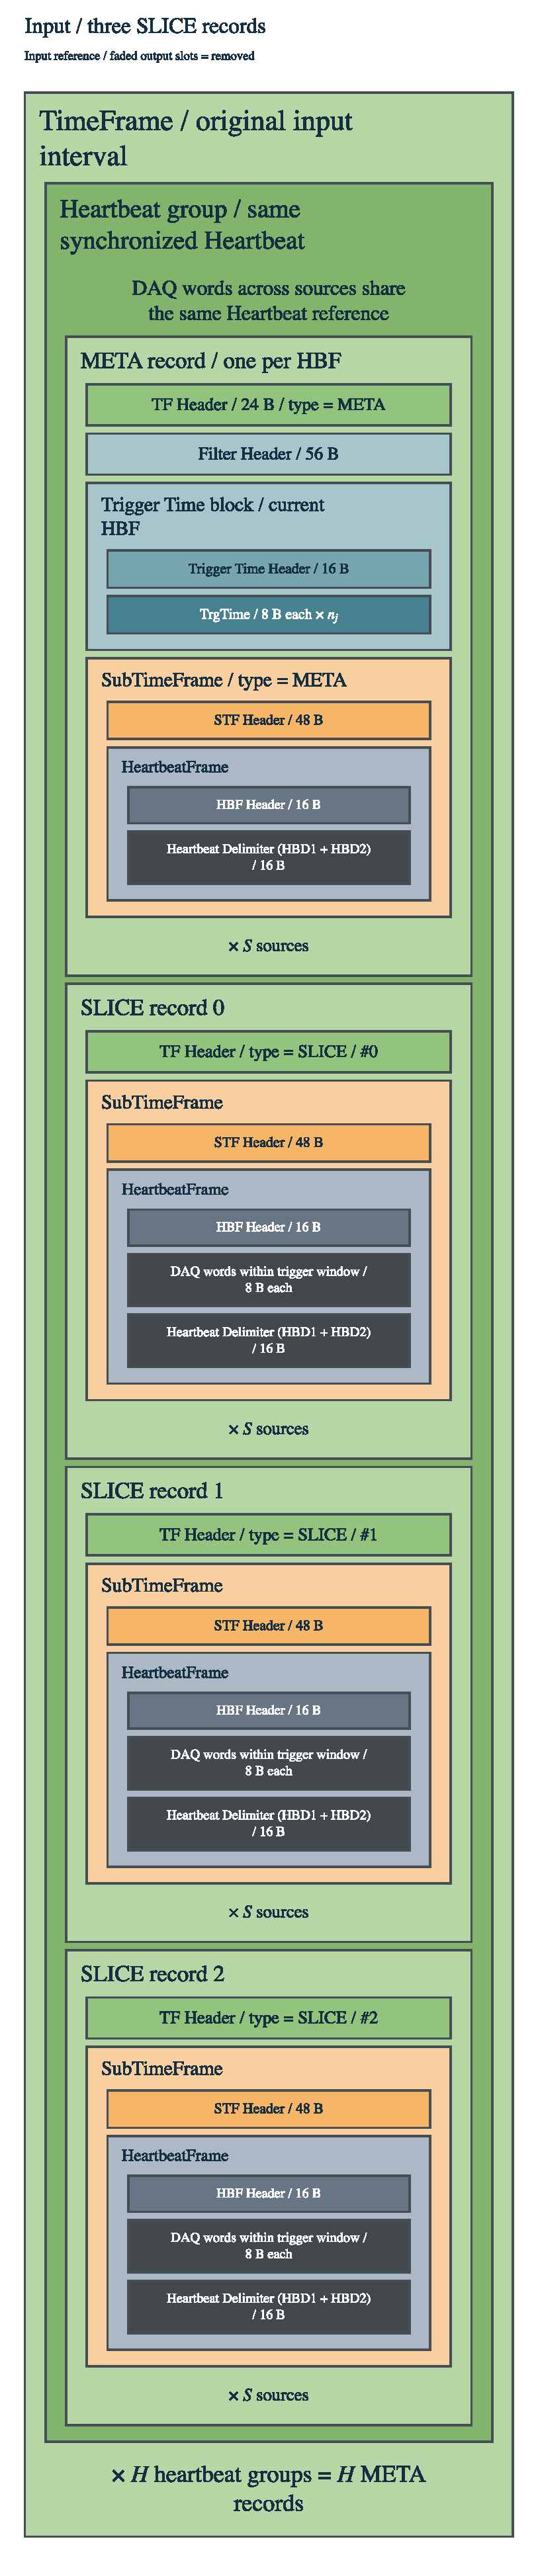
\includegraphics[pagebox=cropbox,width=0.95\linewidth,height=0.70\textheight,keepaspectratio]{../figure/10-3-nestdaq-dataformat/pdf/07-filter-input.pdf}}
\caption{入力：3個のSLICE}\label{fig:format-svg-07-filter-input}\end{figure}

図\ref{fig:format-svg-07-filter-output}に示す。
\begin{figure}[htbp]\centering
\makebox[\linewidth][c]{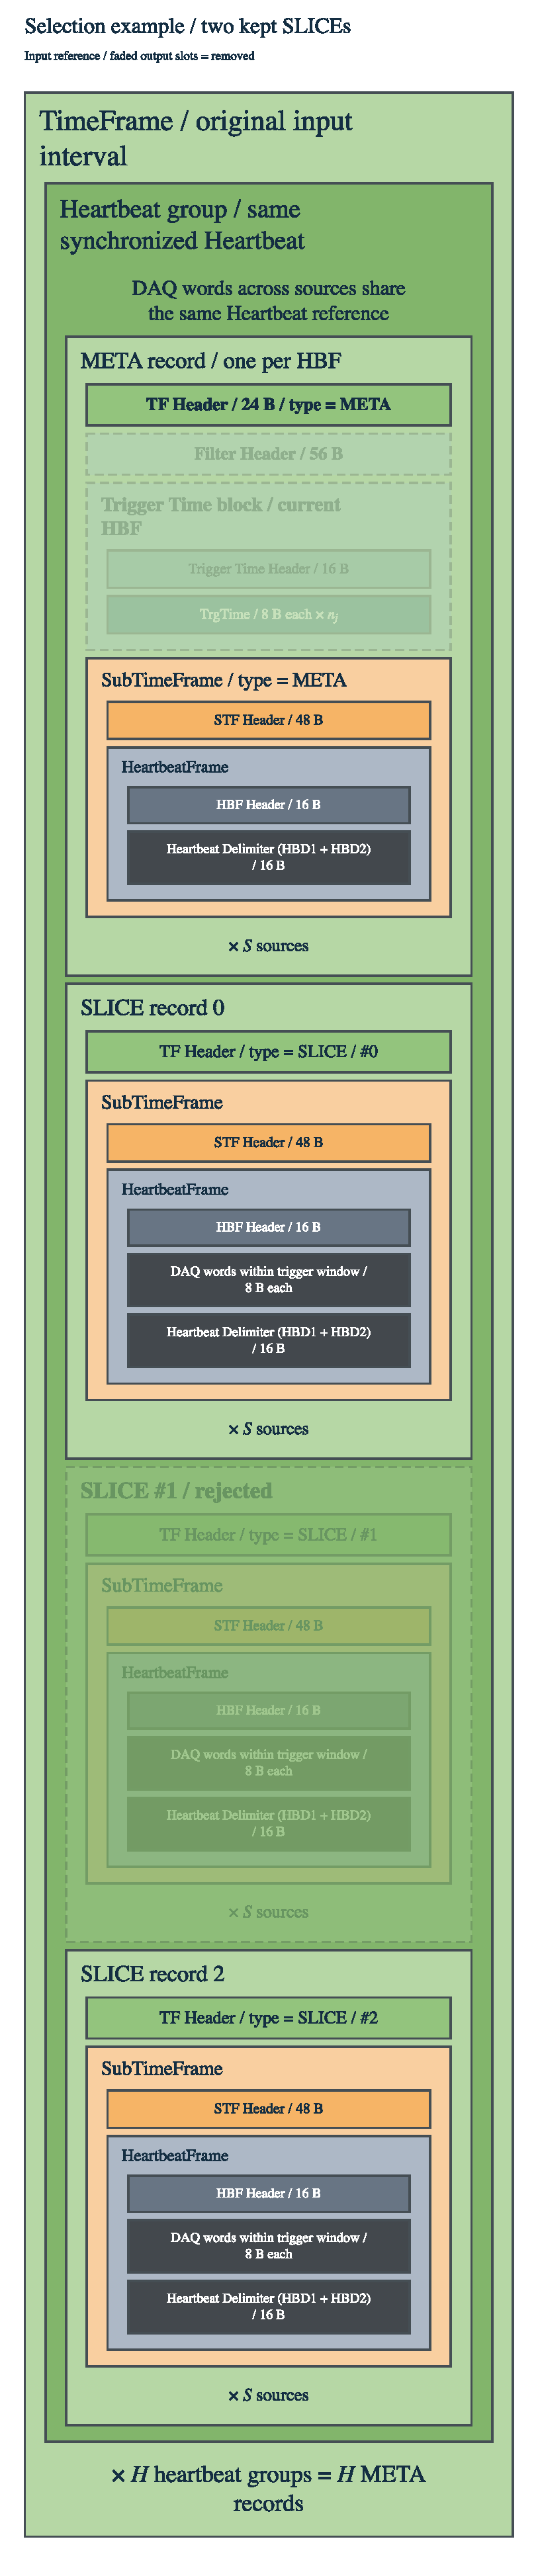
\includegraphics[pagebox=cropbox,width=0.95\linewidth,height=0.70\textheight,keepaspectratio]{../figure/10-3-nestdaq-dataformat/pdf/07-filter-output.pdf}}
\caption{選別例：SLICE \#1を除去}\label{fig:format-svg-07-filter-output}\end{figure}

\subsubsection{FileSink}
入力順にTF列を書き、ファイル先頭と末尾へ304 byteのFileSink Header/Trailerを付ける。図は非圧縮の論理byte列。

非圧縮の論理byte列は \texttt{[FileSink Header] [META TF] [採用SLICE TF列] [次のMETA TF] … [FileSink Trailer]}。入力の順序を保つ。multipartのpart境界を示す別のレコードはこの書き込み経路では付けず、連結して書く（WriteMultipartData）。読出しは各ヘッダのmagicとlengthなどで構造をたどる。

FileSink Header/Trailerはtime\_t=8 byteの環境で各304 byte。同じフィールド配置だがmagicが違い、HeaderのstopUnixtimeは0、Trailerには終了時刻が入る（Headerの設定、Trailerの設定）。圧縮やファイル分割を有効にした場合は、保存ファイルの物理構造をその設定と併せて読む。


図\ref{fig:format-svg-08-filesink}に示す。
\begin{figure}[htbp]\centering
\makebox[\linewidth][c]{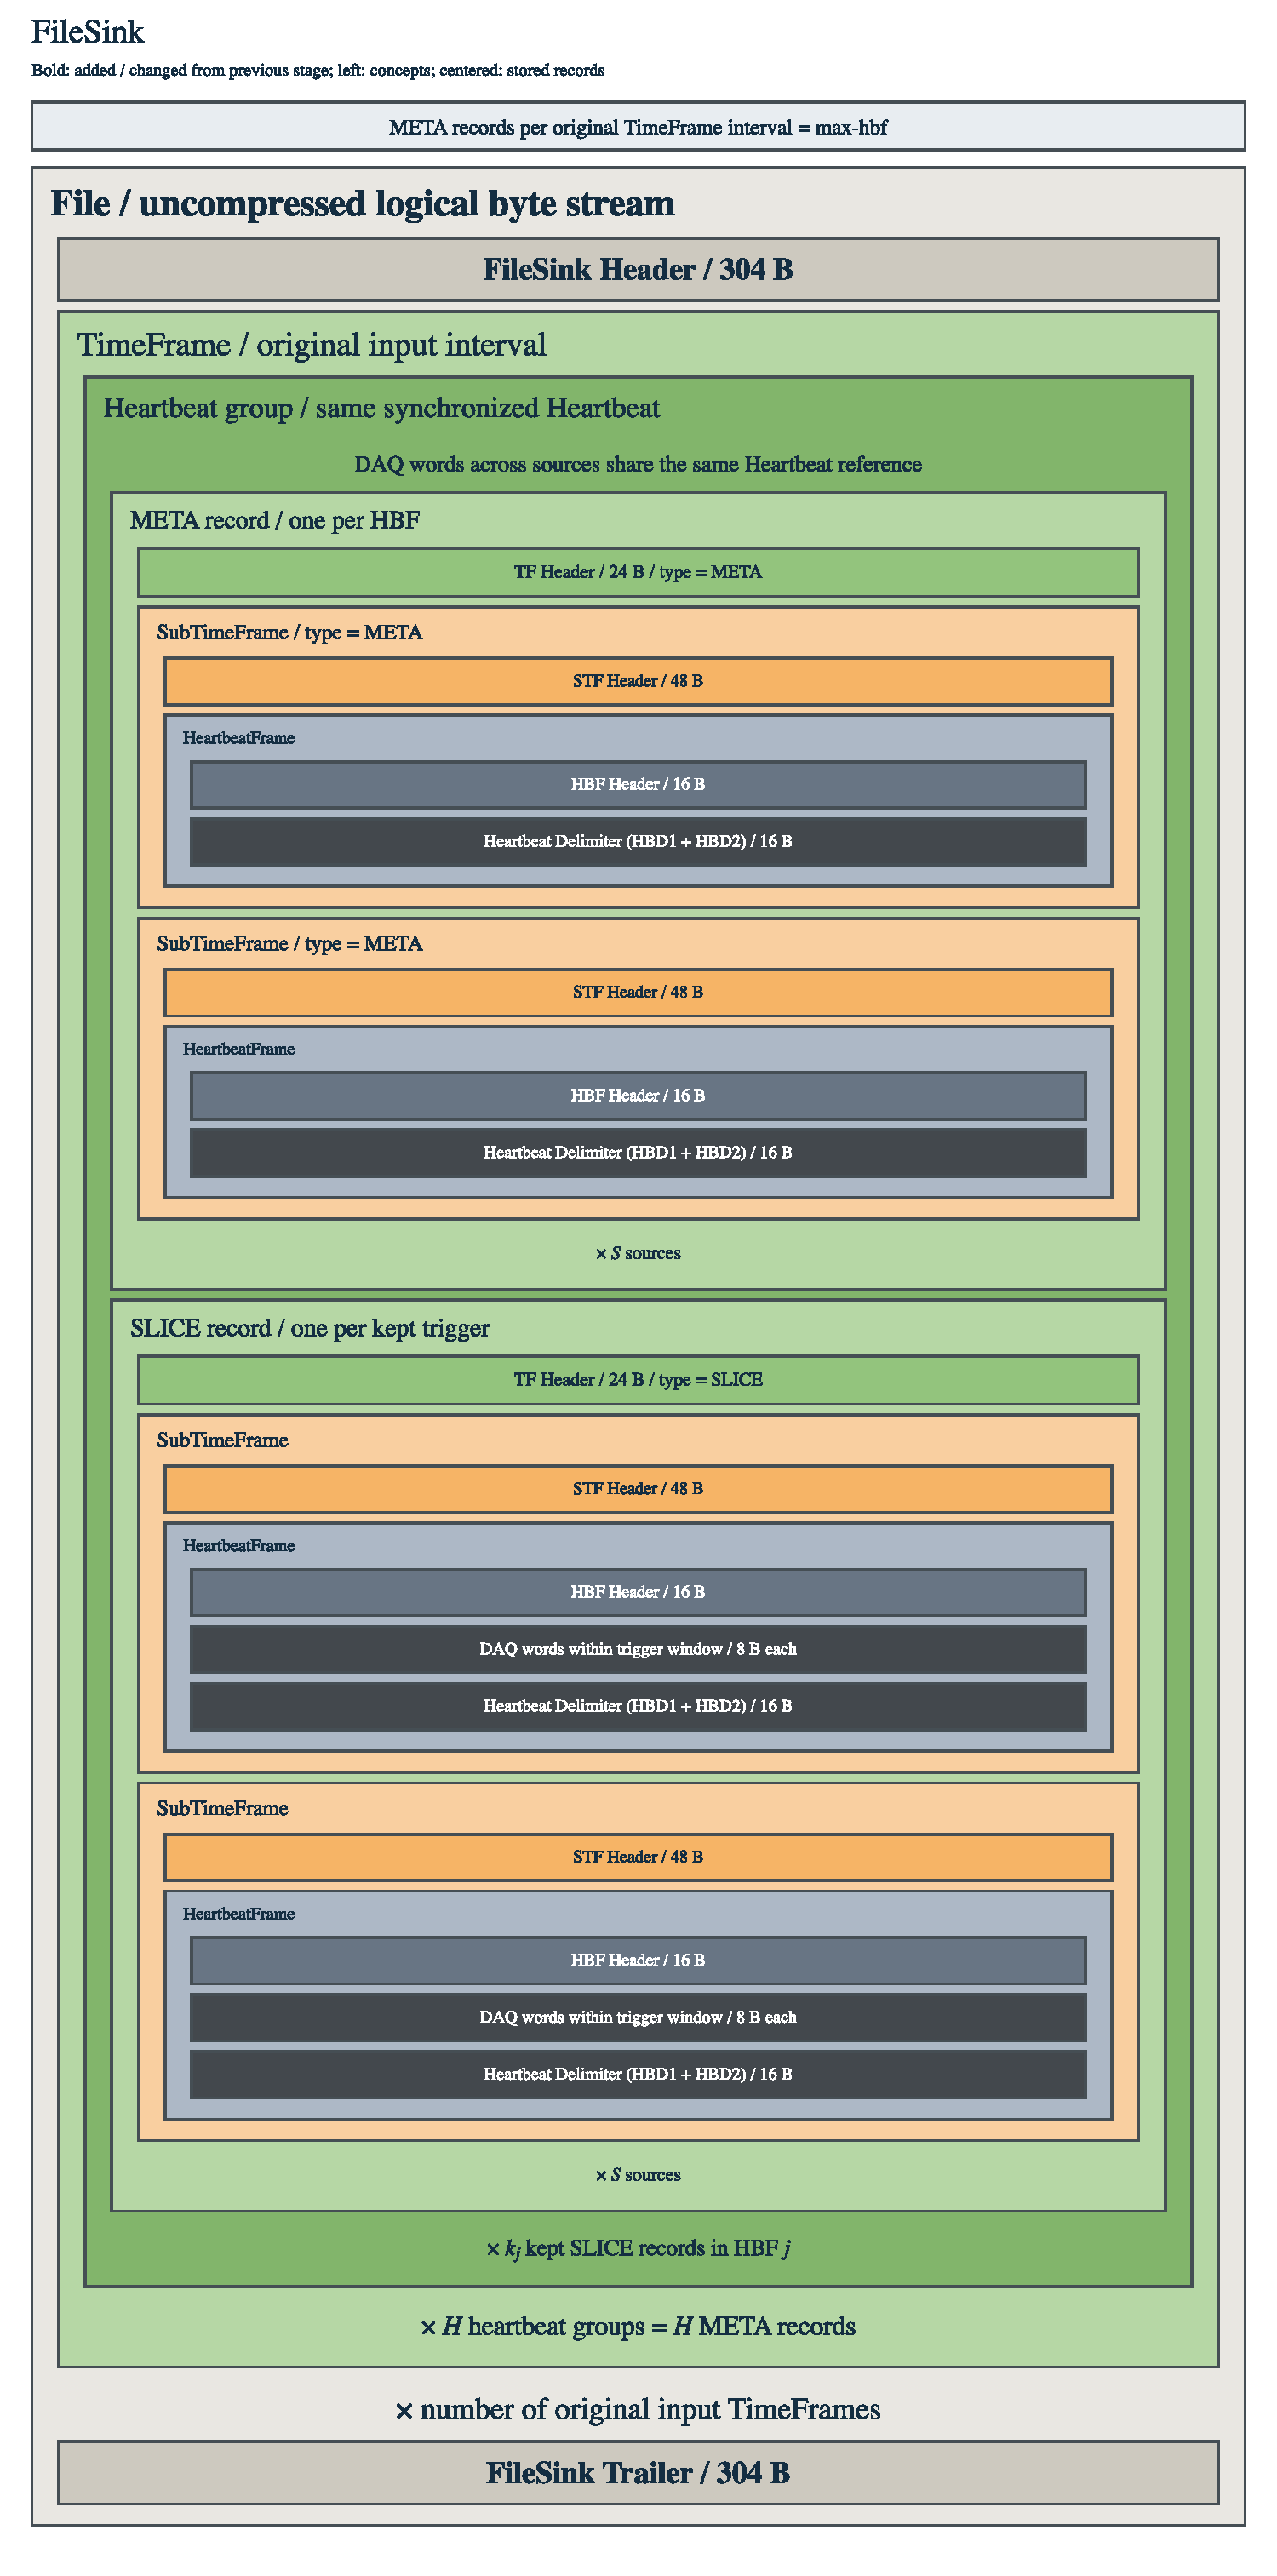
\includegraphics[pagebox=cropbox,width=0.95\linewidth,height=0.70\textheight,keepaspectratio]{../figure/10-3-nestdaq-dataformat/pdf/08-filesink.pdf}}
\caption{FileSinkの出力。}\label{fig:format-svg-08-filesink}\end{figure}

\FloatBarrier
\subsection{ヘッダ・レコード定義とmagic}
\label{sec:format-html-headers}
magicはuint64\_tの定数値と、\textbf{little-endianでメモリ／ファイルに並べた8 byteの文字表現}を示す。\texttt{\textbackslash{}0}は実byte 0x00。コードコメントの末尾空白と、実定数のNULは区別する。ASCII表現はC文字列として途中で打ち切らず8 byteで読む。


\FloatBarrier
{\footnotesize\setlength{\tabcolsep}{3pt}\begin{longtable}{p{0.22\linewidth}p{0.06\linewidth}p{0.22\linewidth}p{0.17\linewidth}p{0.2\linewidth}}
\caption{ヘッダ・レコード定義とmagic。}\label{tab:format-html-2}\\
\hline
構造体 & size [B] & magic [hex] & 8 byteの文字表現（LE） & 実byte [hex] \\ \hline\endfirsthead
\hline 構造体 & size [B] & magic [hex] & 8 byteの文字表現（LE） & 実byte [hex] \\ \hline\endhead
{TimeFrame::v1::Header} & {24} & {\texttt{0x004d5246454d4954}} & {\texttt{"TIMEFRM\textbackslash{}0"}} & {\texttt{54 49 4d 45 46 52 4d 00}} \\
{SubTimeFrame::v1::Header} & {48} & {\texttt{0x00454d4954425553}} & {\texttt{"SUBTIME\textbackslash{}0"}} & {\texttt{53 55 42 54 49 4d 45 00}} \\
{HeartbeatFrame::Header} & {16} & {\texttt{0x0054414542545248}} & {\texttt{"HRTBEAT\textbackslash{}0"}} & {\texttt{48 52 54 42 45 41 54 00}} \\
{Filter::v1::Header} & {56} & {\texttt{0x0049474f4c544c46}} & {\texttt{"FLTLOGI\textbackslash{}0"}} & {\texttt{46 4c 54 4c 4f 47 49 00}} \\
{Filter::v1::TrgTimeHeader} & {16} & {\texttt{0x00454d4954475254}} & {\texttt{"TRGTIME\textbackslash{}0"}} & {\texttt{54 52 47 54 49 4d 45 00}} \\
{FileSinkHeader::v1::Header} & {304} & {\texttt{0x004b4e53454c4946}} & {\texttt{"FILESNK\textbackslash{}0"}} & {\texttt{46 49 4c 45 53 4e 4b 00}} \\
{FileSinkTrailer::v1::Trailer} & {304} & {\texttt{0x004c5254454c4946}} & {\texttt{"FILETRL\textbackslash{}0"}} & {\texttt{46 49 4c 45 54 52 4c 00}} \\
{Filter::v1::TrgTime} & {8} & {なし} & {なし} & {—} \\
\hline\end{longtable}}
この環境のclang++で全構造体のsizeofと全フィールドのoffsetofを検査済み（64項目）。。別のABIや旧版ファイルの配置まで保証するものではない。byte図はアドレス順、bit図はMSB$\rightarrow$LSBで読む。


\clearpage
\subsubsection{TimeFrame::v1::Header / 24 byte}
根拠：TimeFrameHeader.h（v1を参照）。


\begin{itemize}
\item META=0x0001、SLICE=0x0002。typeの上位8 bitはframework用、下位8 bitは実験用。
\item frameworkフラグ：INCOMPLETE=0x8000、TIMEOUT=0x4000、DEPTH\_LIMIT=0x2000。TF\_COMPLETE=0。
\end{itemize}

\FloatBarrier
{\footnotesize\setlength{\tabcolsep}{3pt}\begin{longtable}{p{0.1\linewidth}p{0.1\linewidth}p{0.29\linewidth}p{0.39\linewidth}}
\caption{TimeFrame::v1::Header / 24 byte。}\label{tab:format-html-3}\\
\hline
offset [B] & size [B] & field / type & 内容 \\ \hline\endfirsthead
\hline offset [B] & size [B] & field / type & 内容 \\ \hline\endhead
{0} & {8} & {\texttt{magic} \texttt{uint64\_\allowbreak{}t}} & {} \\
{8} & {4} & {\texttt{length} \texttt{uint32\_\allowbreak{}t}} & {自分のヘッダを含むフレーム長 [byte]} \\
{12} & {2} & {\texttt{hLength} \texttt{uint16\_\allowbreak{}t}} & {ヘッダ長 [byte]} \\
{14} & {2} & {\texttt{type} \texttt{uint16\_\allowbreak{}t}} & {} \\
{16} & {4} & {\texttt{timeFrameId} \texttt{uint32\_\allowbreak{}t}} & {集約するSTFと対応するID} \\
{20} & {4} & {\texttt{numSource} \texttt{uint32\_\allowbreak{}t}} & {TFに含めるソース数} \\
\hline\end{longtable}}

図\ref{fig:format-svg-tf-bytes}に示す。
\begin{figure}[htbp]\centering
\makebox[\linewidth][c]{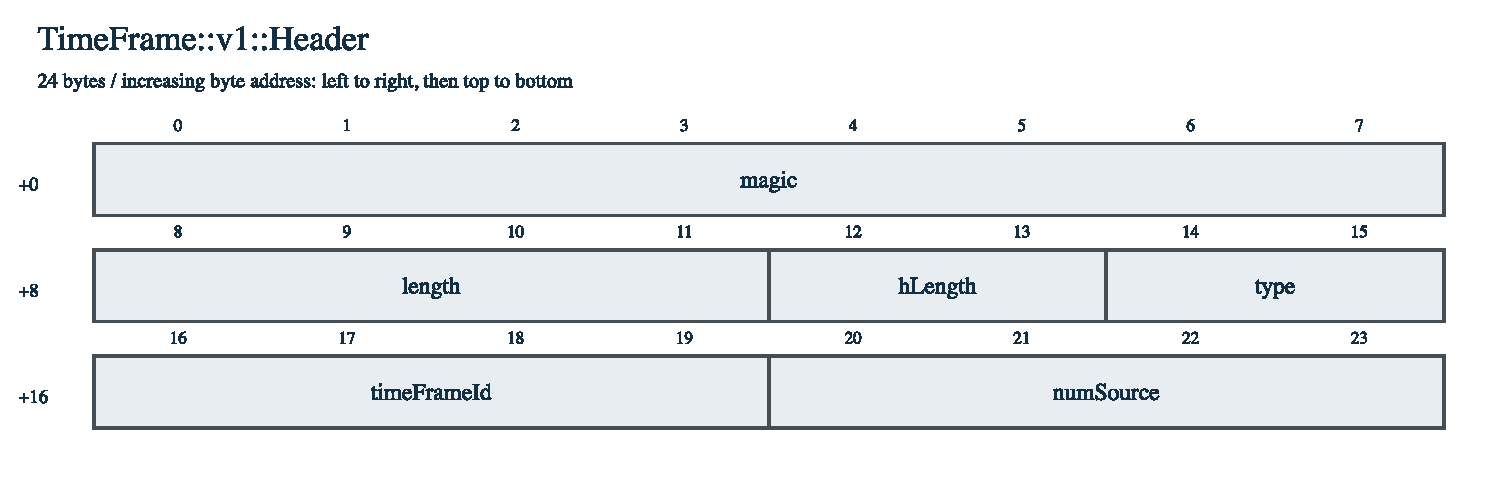
\includegraphics[pagebox=cropbox,width=0.95\linewidth,height=0.70\textheight,keepaspectratio]{../figure/10-3-nestdaq-dataformat/pdf/tf-bytes.pdf}}
\caption{TimeFrame::v1::Headerのバイト配置}\label{fig:format-svg-tf-bytes}\end{figure}

\clearpage
\subsubsection{SubTimeFrame::v1::Header / 48 byte}
根拠：SubTimeFrameHeader.h（v1を参照）。


\begin{itemize}
\item META=1。STFBuilderはtypeにthrottling状態を設定する。段階に応じた意味を読むこと。
\item femType：NULDEV=0、TDC64L\_V1=1、TDC64H/V1=2、TDC64L/V2=3、TDC64H\_V3=5、TDC64L\_V3=6、INPUT\_REG=21、FLT\_TDC=0x1000。
\item SlicerのSLICEではnumMessages=2が書かれる。常にHBF数と同一とみなすことはできない。
\end{itemize}

\FloatBarrier
{\footnotesize\setlength{\tabcolsep}{3pt}\begin{longtable}{p{0.1\linewidth}p{0.1\linewidth}p{0.29\linewidth}p{0.39\linewidth}}
\caption{SubTimeFrame::v1::Header / 48 byte。}\label{tab:format-html-4}\\
\hline
offset [B] & size [B] & field / type & 内容 \\ \hline\endfirsthead
\hline offset [B] & size [B] & field / type & 内容 \\ \hline\endhead
{0} & {8} & {\texttt{magic} \texttt{uint64\_\allowbreak{}t}} & {} \\
{8} & {4} & {\texttt{length} \texttt{uint32\_\allowbreak{}t}} & {自分のヘッダを含むフレーム長 [byte]} \\
{12} & {2} & {\texttt{hLength} \texttt{uint16\_\allowbreak{}t}} & {ヘッダ長 [byte]} \\
{14} & {2} & {\texttt{type} \texttt{uint16\_\allowbreak{}t}} & {} \\
{16} & {4} & {\texttt{timeFrameId} \texttt{uint32\_\allowbreak{}t}} & {STFBuilderの設定によりHBD由来IDまたは連番} \\
{20} & {4} & {\texttt{femType} \texttt{uint32\_\allowbreak{}t}} & {FEM種別・データ世代の識別} \\
{24} & {4} & {\texttt{femId} \texttt{uint32\_\allowbreak{}t}} & {FEM識別子} \\
{28} & {4} & {\texttt{numMessages} \texttt{uint32\_\allowbreak{}t}} & {STFBuilderではSTFヘッダを除くpayloadメッセージ数} \\
{32} & {8} & {\texttt{timeSec} \texttt{uint64\_\allowbreak{}t}} & {STFBuilderではgettimeofday().tv\_sec} \\
{40} & {8} & {\texttt{timeUSec} \texttt{uint64\_\allowbreak{}t}} & {STFBuilderではgettimeofday().tv\_usec：秒内の$\mu$s} \\
\hline\end{longtable}}

図\ref{fig:format-svg-stf-bytes}に示す。
\begin{figure}[htbp]\centering
\makebox[\linewidth][c]{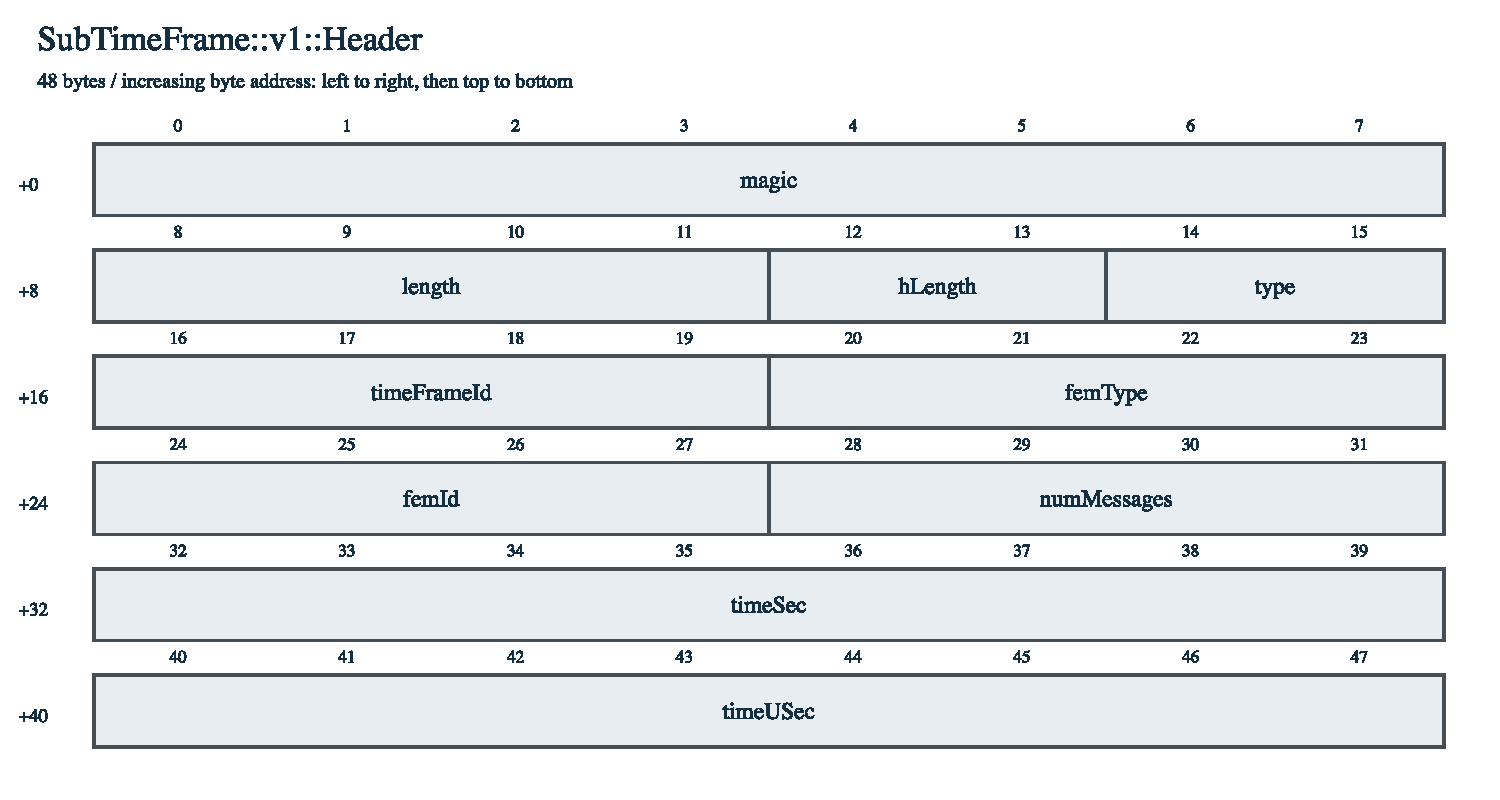
\includegraphics[pagebox=cropbox,width=0.95\linewidth,height=0.70\textheight,keepaspectratio]{../figure/10-3-nestdaq-dataformat/pdf/stf-bytes.pdf}}
\caption{SubTimeFrame::v1::Headerのバイト配置}\label{fig:format-svg-stf-bytes}\end{figure}

\clearpage
\subsubsection{HeartbeatFrame::Header / 16 byte}
根拠：HeartbeatFrameHeader.h。


\begin{itemize}
\item STFBuilder内の別定義HBFHeaderも同じ先頭16 byte配置。offset 14はreserveという名前で0に初期化される。
\item HBFと末尾のHeartbeat Delimiter（HBD）は別物。HBF Headerはソフトウェア側、HBDはFEEデータ中の区切り。
\end{itemize}

\FloatBarrier
{\footnotesize\setlength{\tabcolsep}{3pt}\begin{longtable}{p{0.1\linewidth}p{0.1\linewidth}p{0.29\linewidth}p{0.39\linewidth}}
\caption{HeartbeatFrame::Header / 16 byte。}\label{tab:format-html-5}\\
\hline
offset [B] & size [B] & field / type & 内容 \\ \hline\endfirsthead
\hline offset [B] & size [B] & field / type & 内容 \\ \hline\endhead
{0} & {8} & {\texttt{magic} \texttt{uint64\_\allowbreak{}t}} & {} \\
{8} & {4} & {\texttt{length} \texttt{uint32\_\allowbreak{}t}} & {自分のヘッダを含むフレーム長 [byte]} \\
{12} & {2} & {\texttt{hLength} \texttt{uint16\_\allowbreak{}t}} & {ヘッダ長 [byte]} \\
{14} & {2} & {\texttt{type} \texttt{uint16\_\allowbreak{}t}} & {} \\
\hline\end{longtable}}

図\ref{fig:format-svg-hbf-bytes}に示す。
\begin{figure}[htbp]\centering
\makebox[\linewidth][c]{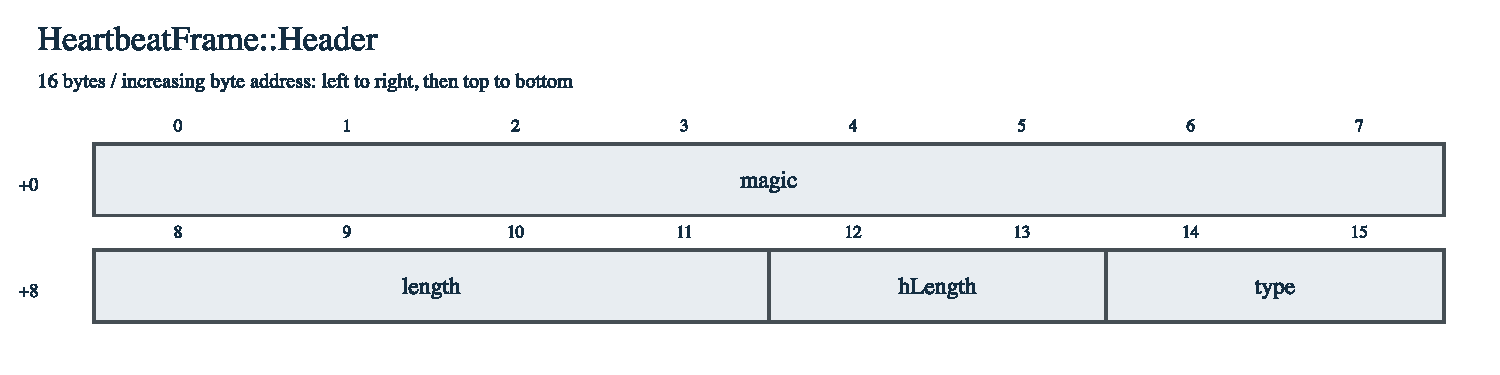
\includegraphics[pagebox=cropbox,width=0.95\linewidth,height=0.70\textheight,keepaspectratio]{../figure/10-3-nestdaq-dataformat/pdf/hbf-bytes.pdf}}
\caption{HeartbeatFrame::Headerのバイト配置}\label{fig:format-svg-hbf-bytes}\end{figure}

\clearpage
\subsubsection{Filter::v1::Header / 56 byte}
根拠：FilterHeader.h（v1を参照）。


\begin{itemize}
\item LogicFilter出力では単一のFilter HeaderとHBF別Trigger Timeブロックが続く。
\item AddFilterMessageのlength計算はTrgTimeを4 byteとして数えているが、実際の出力は8 byte。資料では宣言値・実際のbyte数を区別する。
\end{itemize}

\FloatBarrier
{\footnotesize\setlength{\tabcolsep}{3pt}\begin{longtable}{p{0.1\linewidth}p{0.1\linewidth}p{0.29\linewidth}p{0.39\linewidth}}
\caption{Filter::v1::Header / 56 byte。}\label{tab:format-html-6}\\
\hline
offset [B] & size [B] & field / type & 内容 \\ \hline\endfirsthead
\hline offset [B] & size [B] & field / type & 内容 \\ \hline\endhead
{0} & {8} & {\texttt{magic} \texttt{uint64\_\allowbreak{}t}} & {} \\
{8} & {4} & {\texttt{length} \texttt{uint32\_\allowbreak{}t}} & {自分のヘッダを含むフレーム長 [byte]} \\
{12} & {2} & {\texttt{hLength} \texttt{uint16\_\allowbreak{}t}} & {ヘッダ長 [byte]} \\
{14} & {2} & {\texttt{type} \texttt{uint16\_\allowbreak{}t}} & {} \\
{16} & {4} & {\texttt{timeFrameId} \texttt{uint32\_\allowbreak{}t}} & {} \\
{20} & {4} & {\texttt{numTrigs} \texttt{uint32\_\allowbreak{}t}} & {LogicFilterでは全HBFのtrigger数の合計} \\
{24} & {4} & {\texttt{workerId} \texttt{uint32\_\allowbreak{}t}} & {} \\
{28} & {4} & {\texttt{numMessages} \texttt{uint32\_\allowbreak{}t}} & {LogicFilterでは1 + Trigger Timeブロック数} \\
{32} & {4} & {\texttt{elapseTime} \texttt{uint32\_\allowbreak{}t}} & {LogicFilterの処理経過時間 [$\mu$s]} \\
{36} & {4} & {\texttt{reserve} \texttt{uint32\_\allowbreak{}t}} & {初期値0xff00ff00} \\
{40} & {8} & {\texttt{timeSec} \texttt{uint64\_\allowbreak{}t}} & {LogicFilterではepochからの秒} \\
{48} & {8} & {\texttt{timeUSec} \texttt{uint64\_\allowbreak{}t}} & {LogicFilterではepochからの総$\mu$s。STFのtimeUSecとは意味が異なる} \\
\hline\end{longtable}}

図\ref{fig:format-svg-filter-bytes}に示す。
\begin{figure}[htbp]\centering
\makebox[\linewidth][c]{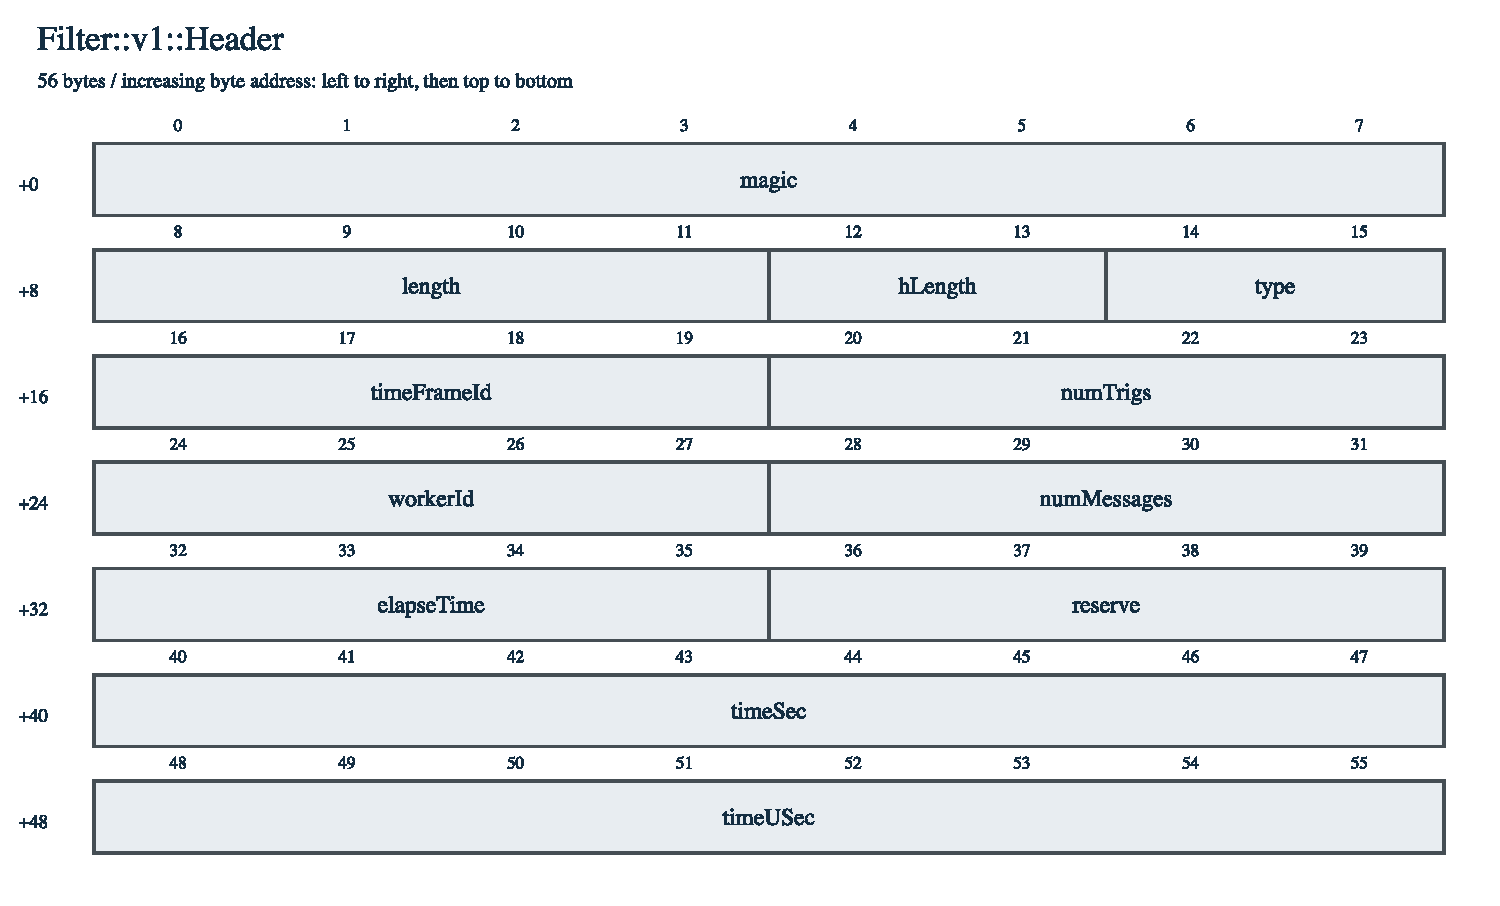
\includegraphics[pagebox=cropbox,width=0.95\linewidth,height=0.70\textheight,keepaspectratio]{../figure/10-3-nestdaq-dataformat/pdf/filter-bytes.pdf}}
\caption{Filter::v1::Headerのバイト配置}\label{fig:format-svg-filter-bytes}\end{figure}

\clearpage
\subsubsection{Filter::v1::TrgTimeHeader / 16 byte}
根拠：FilterHeader.h（v1を参照）。


\begin{itemize}
\item 直後にTrgTimeがN個続く。length=16+8N。Trigger数が0でも16 byteのHeaderはあり得る。
\end{itemize}

\FloatBarrier
{\footnotesize\setlength{\tabcolsep}{3pt}\begin{longtable}{p{0.1\linewidth}p{0.1\linewidth}p{0.29\linewidth}p{0.39\linewidth}}
\caption{Filter::v1::TrgTimeHeader / 16 byte。}\label{tab:format-html-7}\\
\hline
offset [B] & size [B] & field / type & 内容 \\ \hline\endfirsthead
\hline offset [B] & size [B] & field / type & 内容 \\ \hline\endhead
{0} & {8} & {\texttt{magic} \texttt{uint64\_\allowbreak{}t}} & {} \\
{8} & {4} & {\texttt{length} \texttt{uint32\_\allowbreak{}t}} & {自分のヘッダを含むフレーム長 [byte]} \\
{12} & {2} & {\texttt{hLength} \texttt{uint16\_\allowbreak{}t}} & {ヘッダ長 [byte]} \\
{14} & {2} & {\texttt{type} \texttt{uint16\_\allowbreak{}t}} & {} \\
\hline\end{longtable}}

図\ref{fig:format-svg-trigger-bytes}に示す。
\begin{figure}[htbp]\centering
\makebox[\linewidth][c]{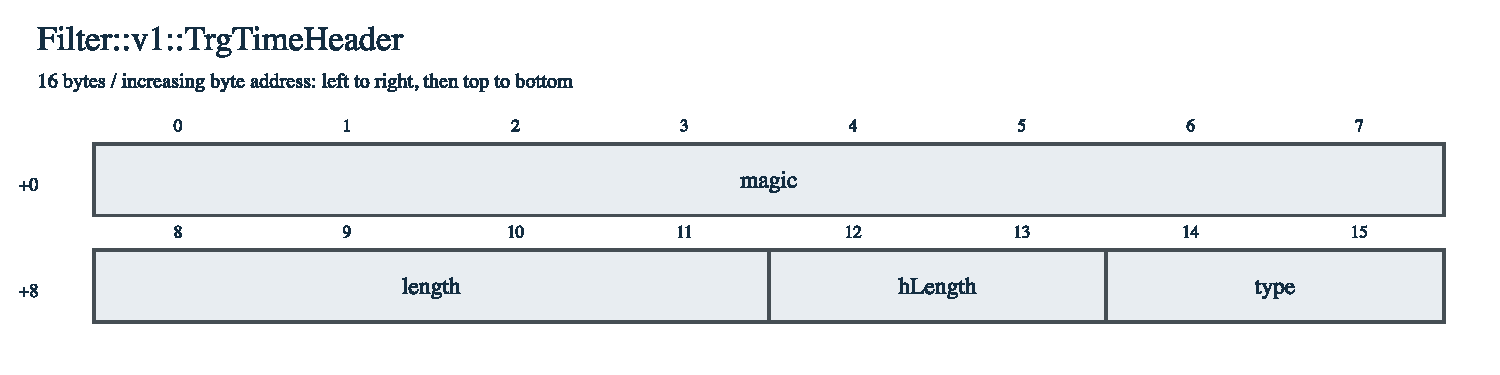
\includegraphics[pagebox=cropbox,width=0.95\linewidth,height=0.70\textheight,keepaspectratio]{../figure/10-3-nestdaq-dataformat/pdf/trigger-bytes.pdf}}
\caption{Filter::v1::TrgTimeHeaderのバイト配置}\label{fig:format-svg-trigger-bytes}\end{figure}

\clearpage
\subsubsection{FileSinkHeader::v1::Header / 304 byte}
根拠：FileSinkHeader.h（v1を参照）。


\begin{itemize}
\item offset 8〜15はuint64\_t sizeとのunion。length / hLength / typeとしても参照する。
\item HeaderとTrailerのレイアウトは同じだが、magicとstopUnixtimeなどの値は異なる。304 byteはtime\_tが8 byteの環境。
\end{itemize}

\FloatBarrier
{\footnotesize\setlength{\tabcolsep}{3pt}\begin{longtable}{p{0.1\linewidth}p{0.1\linewidth}p{0.29\linewidth}p{0.39\linewidth}}
\caption{FileSinkHeader::v1::Header / 304 byte。}\label{tab:format-html-8}\\
\hline
offset [B] & size [B] & field / type & 内容 \\ \hline\endfirsthead
\hline offset [B] & size [B] & field / type & 内容 \\ \hline\endhead
{0} & {8} & {\texttt{magic} \texttt{uint64\_\allowbreak{}t}} & {} \\
{8} & {4} & {\texttt{length} \texttt{uint32\_\allowbreak{}t}} & {自分のヘッダを含むフレーム長 [byte]} \\
{12} & {2} & {\texttt{hLength} \texttt{uint16\_\allowbreak{}t}} & {ヘッダ長 [byte]} \\
{14} & {2} & {\texttt{type} \texttt{uint16\_\allowbreak{}t}} & {} \\
{16} & {8} & {\texttt{fairMQDeviceType} \texttt{uint64\_\allowbreak{}t}} & {FileSinkのHeaderで99に設定} \\
{24} & {8} & {\texttt{runNumber} \texttt{uint64\_\allowbreak{}t}} & {} \\
{32} & {8} & {\texttt{startUnixtime} \texttt{time\_\allowbreak{}t}} & {run開始時刻。ここではtime\_t=8を仮定} \\
{40} & {8} & {\texttt{stopUnixtime} \texttt{time\_\allowbreak{}t}} & {Headerでは0、Trailerでは終了時刻} \\
{48} & {256} & {\texttt{comments} \texttt{char[256]}} & {runコメント} \\
\hline\end{longtable}}

図\ref{fig:format-svg-file-header-bytes}に示す。
\begin{figure}[htbp]\centering
\makebox[\linewidth][c]{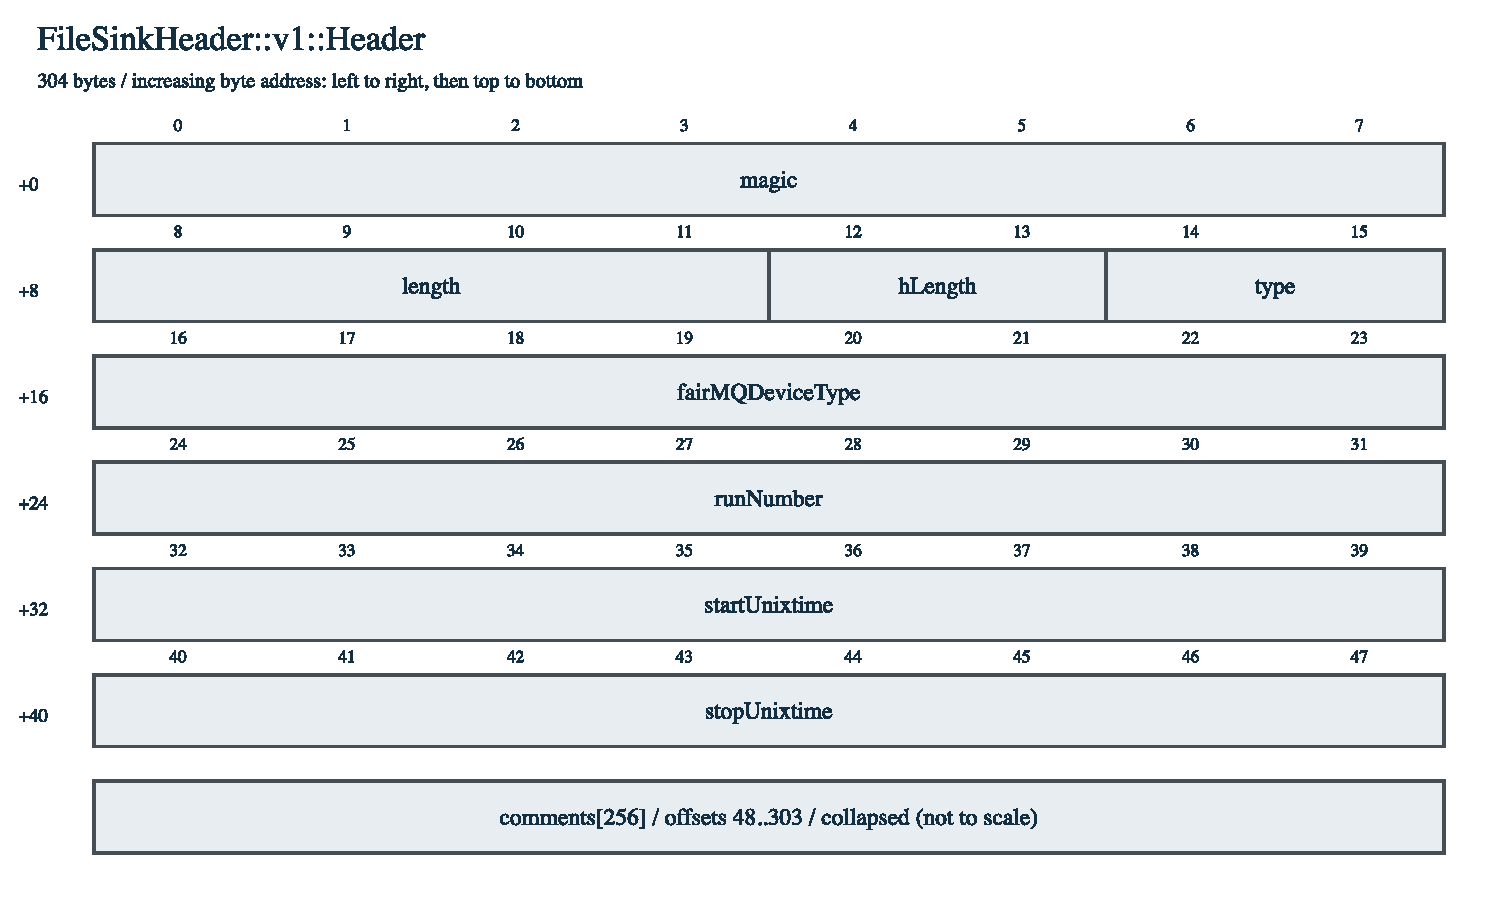
\includegraphics[pagebox=cropbox,width=0.95\linewidth,height=0.70\textheight,keepaspectratio]{../figure/10-3-nestdaq-dataformat/pdf/file-header-bytes.pdf}}
\caption{FileSinkHeader::v1::Headerのバイト配置}\label{fig:format-svg-file-header-bytes}\end{figure}

\clearpage
\subsubsection{FileSinkTrailer::v1::Trailer / 304 byte}
根拠：FileSinkTrailer.h（v1を参照）。


\begin{itemize}
\item offset 8〜15はuint64\_t sizeとのunion。length / hLength / typeとしても参照する。
\item HeaderとTrailerのレイアウトは同じだが、magicとstopUnixtimeなどの値は異なる。304 byteはtime\_tが8 byteの環境。
\end{itemize}

\FloatBarrier
{\footnotesize\setlength{\tabcolsep}{3pt}\begin{longtable}{p{0.1\linewidth}p{0.1\linewidth}p{0.29\linewidth}p{0.39\linewidth}}
\caption{FileSinkTrailer::v1::Trailer / 304 byte。}\label{tab:format-html-9}\\
\hline
offset [B] & size [B] & field / type & 内容 \\ \hline\endfirsthead
\hline offset [B] & size [B] & field / type & 内容 \\ \hline\endhead
{0} & {8} & {\texttt{magic} \texttt{uint64\_\allowbreak{}t}} & {} \\
{8} & {4} & {\texttt{length} \texttt{uint32\_\allowbreak{}t}} & {自分のヘッダを含むフレーム長 [byte]} \\
{12} & {2} & {\texttt{hLength} \texttt{uint16\_\allowbreak{}t}} & {ヘッダ長 [byte]} \\
{14} & {2} & {\texttt{type} \texttt{uint16\_\allowbreak{}t}} & {} \\
{16} & {8} & {\texttt{fairMQDeviceType} \texttt{uint64\_\allowbreak{}t}} & {FileSinkのHeaderで99に設定} \\
{24} & {8} & {\texttt{runNumber} \texttt{uint64\_\allowbreak{}t}} & {} \\
{32} & {8} & {\texttt{startUnixtime} \texttt{time\_\allowbreak{}t}} & {run開始時刻。ここではtime\_t=8を仮定} \\
{40} & {8} & {\texttt{stopUnixtime} \texttt{time\_\allowbreak{}t}} & {Headerでは0、Trailerでは終了時刻} \\
{48} & {256} & {\texttt{comments} \texttt{char[256]}} & {runコメント} \\
\hline\end{longtable}}

図\ref{fig:format-svg-file-trailer-bytes}に示す。
\begin{figure}[htbp]\centering
\makebox[\linewidth][c]{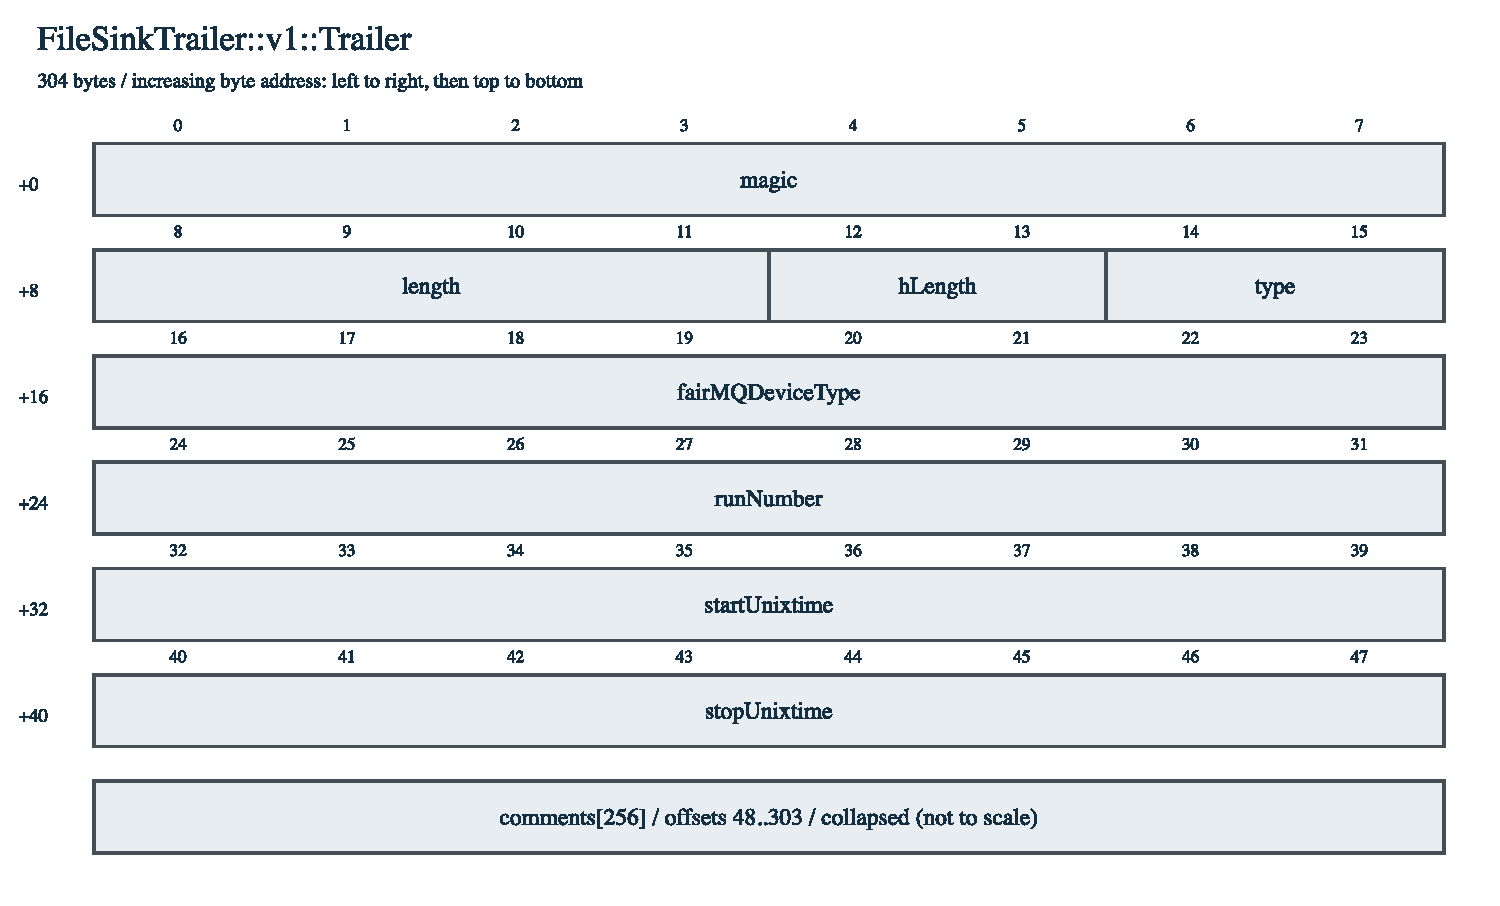
\includegraphics[pagebox=cropbox,width=0.95\linewidth,height=0.70\textheight,keepaspectratio]{../figure/10-3-nestdaq-dataformat/pdf/file-trailer-bytes.pdf}}
\caption{FileSinkTrailer::v1::Trailerのバイト配置}\label{fig:format-svg-file-trailer-bytes}\end{figure}

\clearpage
\subsubsection{Filter::v1::TrgTime / 8 byte}
根拠：FilterHeader.h（v1を参照）。


\begin{itemize}
\item magicは持たない。各レコードは8 byte。timeの比較単位は4 ns系（tdc4n）。
\end{itemize}

\FloatBarrier
{\footnotesize\setlength{\tabcolsep}{3pt}\begin{longtable}{p{0.1\linewidth}p{0.1\linewidth}p{0.29\linewidth}p{0.39\linewidth}}
\caption{Filter::v1::TrgTime / 8 byte。}\label{tab:format-html-10}\\
\hline
offset [B] & size [B] & field / type & 内容 \\ \hline\endfirsthead
\hline offset [B] & size [B] & field / type & 内容 \\ \hline\endhead
{0} & {4} & {\texttt{time} \texttt{uint32\_\allowbreak{}t}} & {trigger時刻。Slicerはtdc4nと比較する} \\
{4} & {4} & {\texttt{type} \texttt{uint32\_\allowbreak{}t}} & {LogicFilterは0xaa000000を出力。little-endian末尾byteは0xaa} \\
\hline\end{longtable}}

図\ref{fig:format-svg-trgtime-bytes}に示す。
\begin{figure}[htbp]\centering
\makebox[\linewidth][c]{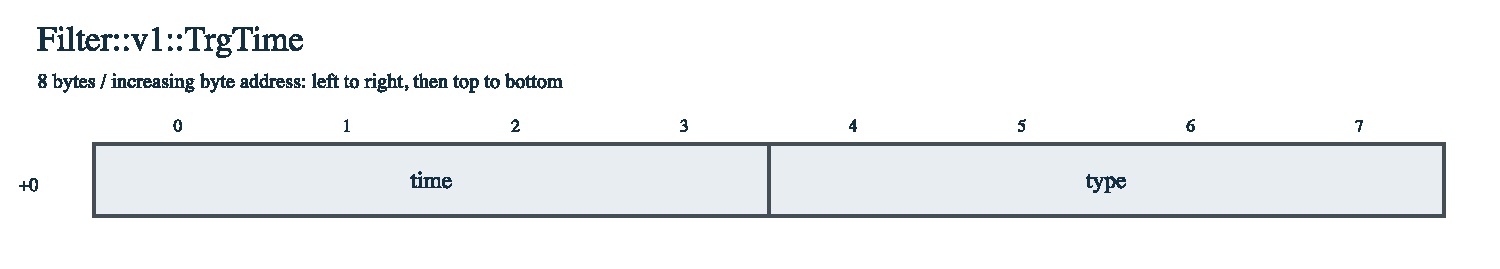
\includegraphics[pagebox=cropbox,width=0.95\linewidth,height=0.70\textheight,keepaspectratio]{../figure/10-3-nestdaq-dataformat/pdf/trgtime-bytes.pdf}}
\caption{Filter::v1::TrgTimeのバイト配置}\label{fig:format-svg-trgtime-bytes}\end{figure}

\FloatBarrier
\subsection{DAQ wordとHeartbeat Delimiter}
\label{sec:format-html-words}
ここではSlicerが処理するTDC64H\_V3 / TDC64L\_V3を対象にする。hitは64 bit＝8 byte。hitのtypeは0x0b（[63:58]）。HBDは2 word＝16 byteで、ソフトウェアのHBF Header 16 byteとは別に存在する。bit抽出の根拠：UnpackTdc.h:296、UnpackTdc.h:383。HBD宣言：AmQStrTdcData.h:111（v1）。


\subsubsection{TDC64H\_V3 / hit}
UnpackTdc.h: tdc4n = TDC >> 12。femType=5。


図\ref{fig:format-svg-hr-v3-bits}に示す。
\begin{figure}[htbp]\centering
\makebox[\linewidth][c]{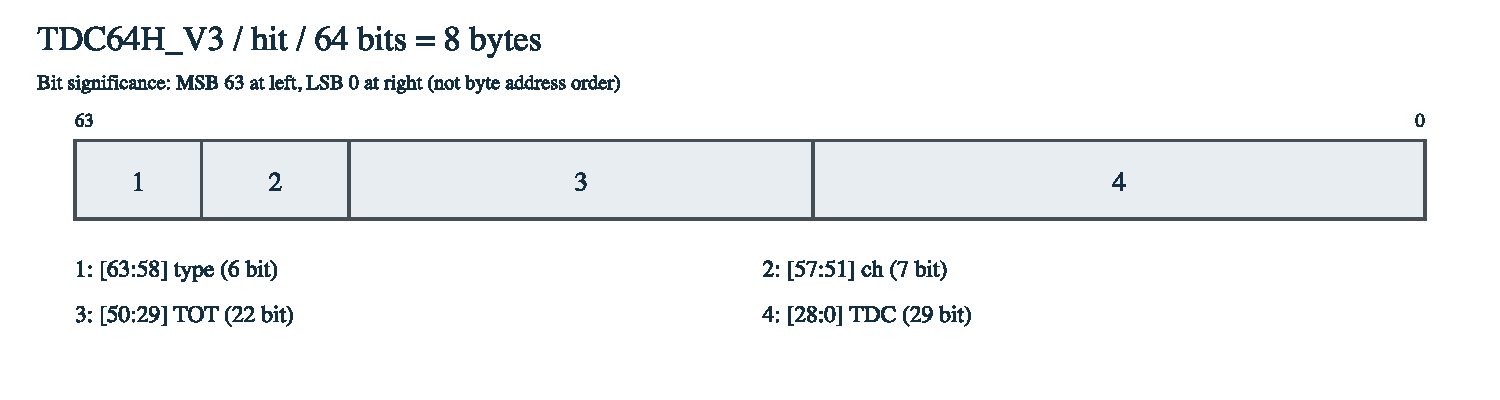
\includegraphics[pagebox=cropbox,width=0.95\linewidth,height=0.70\textheight,keepaspectratio]{../figure/10-3-nestdaq-dataformat/pdf/hr-v3-bits.pdf}}
\caption{TDC64H\_V3 / hitのビット配置}\label{fig:format-svg-hr-v3-bits}\end{figure}

\FloatBarrier
{\footnotesize\setlength{\tabcolsep}{3pt}\begin{longtable}{p{0.3\linewidth}p{0.12\linewidth}p{0.48\linewidth}}
\caption{TDC64H\_V3 / hit。}\label{tab:format-html-11}\\
\hline
bit範囲 & 幅 & field \\ \hline\endfirsthead
\hline bit範囲 & 幅 & field \\ \hline\endhead
{[63:58]} & {6} & {type} \\
{[57:51]} & {7} & {ch} \\
{[50:29]} & {22} & {TOT} \\
{[28:0]} & {29} & {TDC} \\
\hline\end{longtable}}

\subsubsection{TDC64L\_V3 / hit}
UnpackTdc.h: tdc4n = TDC >> 2。femType=6。


図\ref{fig:format-svg-lr-v3-bits}に示す。
\begin{figure}[htbp]\centering
\makebox[\linewidth][c]{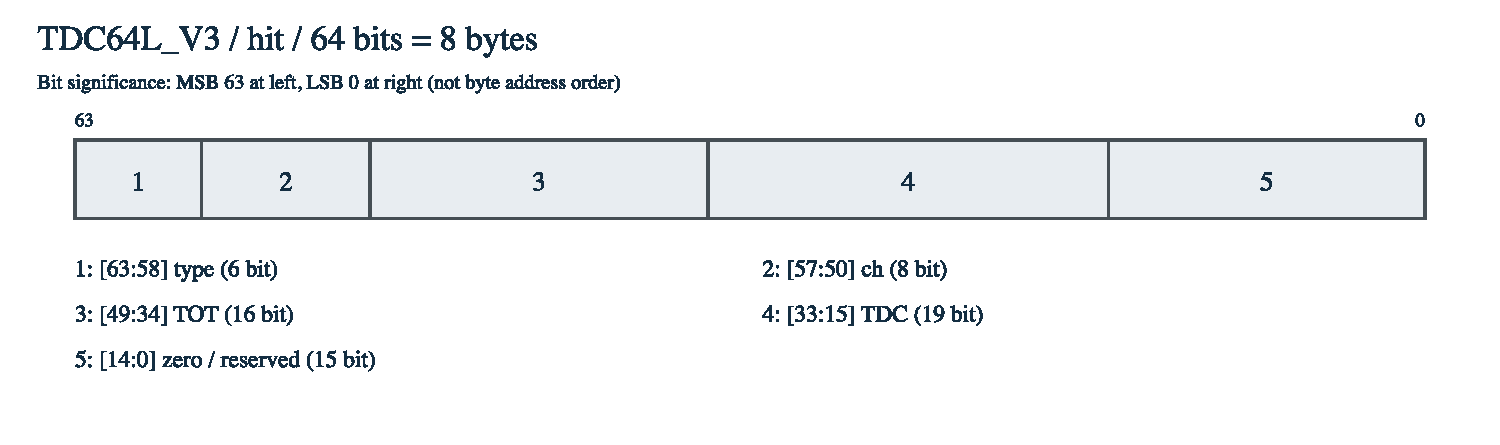
\includegraphics[pagebox=cropbox,width=0.95\linewidth,height=0.70\textheight,keepaspectratio]{../figure/10-3-nestdaq-dataformat/pdf/lr-v3-bits.pdf}}
\caption{TDC64L\_V3 / hitのビット配置}\label{fig:format-svg-lr-v3-bits}\end{figure}

\FloatBarrier
{\footnotesize\setlength{\tabcolsep}{3pt}\begin{longtable}{p{0.3\linewidth}p{0.12\linewidth}p{0.48\linewidth}}
\caption{TDC64L\_V3 / hit。}\label{tab:format-html-12}\\
\hline
bit範囲 & 幅 & field \\ \hline\endfirsthead
\hline bit範囲 & 幅 & field \\ \hline\endhead
{[63:58]} & {6} & {type} \\
{[57:50]} & {8} & {ch} \\
{[49:34]} & {16} & {TOT} \\
{[33:15]} & {19} & {TDC} \\
{[14:0]} & {15} & {zero / reserved} \\
\hline\end{longtable}}

\subsubsection{Heartbeat Delimiter / 1st word}
AmQStrTdcData.h v1。UnpackTdc.h V3はflag、toffset、hartbeatを抽出する。


図\ref{fig:format-svg-hbd1-bits}に示す。
\begin{figure}[htbp]\centering
\makebox[\linewidth][c]{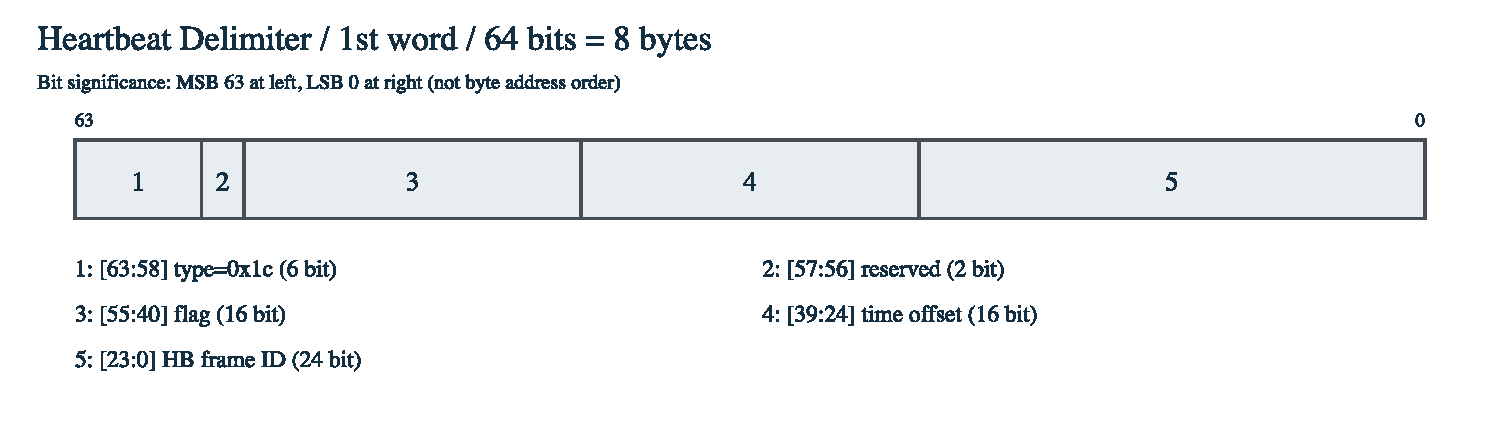
\includegraphics[pagebox=cropbox,width=0.95\linewidth,height=0.70\textheight,keepaspectratio]{../figure/10-3-nestdaq-dataformat/pdf/hbd1-bits.pdf}}
\caption{Heartbeat Delimiter / 1st wordのビット配置}\label{fig:format-svg-hbd1-bits}\end{figure}

\FloatBarrier
{\footnotesize\setlength{\tabcolsep}{3pt}\begin{longtable}{p{0.3\linewidth}p{0.12\linewidth}p{0.48\linewidth}}
\caption{Heartbeat Delimiter / 1st word。}\label{tab:format-html-13}\\
\hline
bit範囲 & 幅 & field \\ \hline\endfirsthead
\hline bit範囲 & 幅 & field \\ \hline\endhead
{[63:58]} & {6} & {type=0x1c} \\
{[57:56]} & {2} & {reserved} \\
{[55:40]} & {16} & {flag} \\
{[39:24]} & {16} & {time offset} \\
{[23:0]} & {24} & {HB frame ID} \\
\hline\end{longtable}}

\subsubsection{Heartbeat Delimiter / 2nd word}
AmQStrTdcData.h v1のフィールド名。V3 unpack側は[55:40]をflagとして読み出す。


図\ref{fig:format-svg-hbd2-bits}に示す。
\begin{figure}[htbp]\centering
\makebox[\linewidth][c]{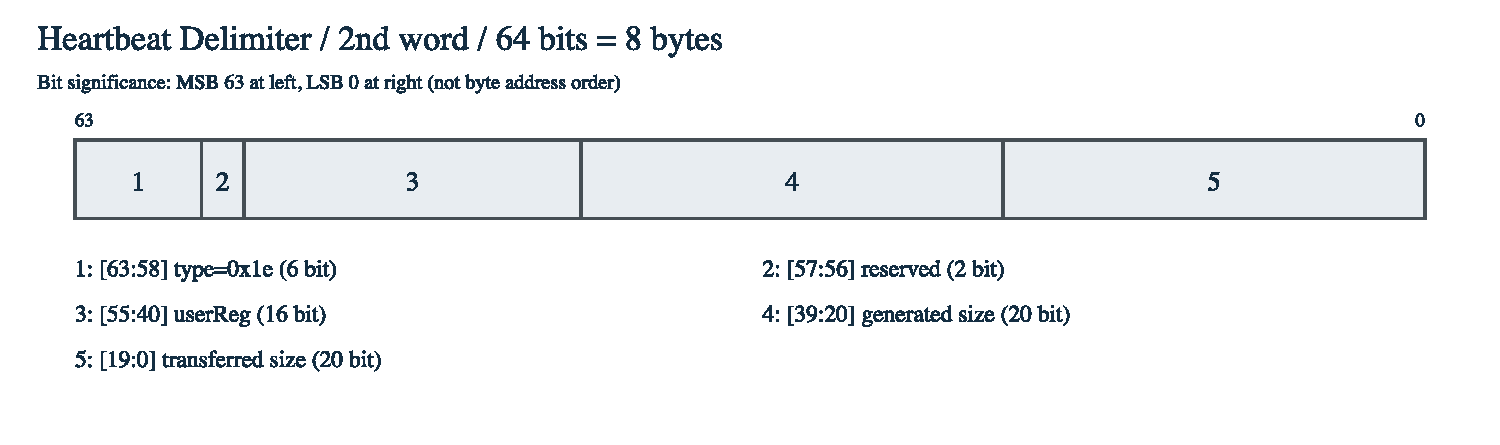
\includegraphics[pagebox=cropbox,width=0.95\linewidth,height=0.70\textheight,keepaspectratio]{../figure/10-3-nestdaq-dataformat/pdf/hbd2-bits.pdf}}
\caption{Heartbeat Delimiter / 2nd wordのビット配置}\label{fig:format-svg-hbd2-bits}\end{figure}

\FloatBarrier
{\footnotesize\setlength{\tabcolsep}{3pt}\begin{longtable}{p{0.3\linewidth}p{0.12\linewidth}p{0.48\linewidth}}
\caption{Heartbeat Delimiter / 2nd word。}\label{tab:format-html-14}\\
\hline
bit範囲 & 幅 & field \\ \hline\endfirsthead
\hline bit範囲 & 幅 & field \\ \hline\endhead
{[63:58]} & {6} & {type=0x1e} \\
{[57:56]} & {2} & {reserved} \\
{[55:40]} & {16} & {userReg} \\
{[39:20]} & {20} & {generated size} \\
{[19:0]} & {20} & {transferred size} \\
\hline\end{longtable}}

\FloatBarrier
\subsection{サイズと個数の関係}
\label{sec:format-html-sizes}
以下はV3のHBDが2 wordで、通常のデータソースだけが存在し、ソースごとにH個のHBFが揃う代表例。D\textsubscript{s,j}をDAQ word数、n\textsubscript{j}をHBF jのtrigger数とする。制御word、既存METAソース、追加情報がある場合はその分を数える。


\FloatBarrier
{\footnotesize\setlength{\tabcolsep}{3pt}\begin{longtable}{p{0.3\linewidth}p{0.12\linewidth}p{0.48\linewidth}}
\caption{サイズと個数の関係。}\label{tab:format-html-15}\\
\hline
対象 & 非圧縮の実byte数 & 意味 \\ \hline\endfirsthead
\hline 対象 & 非圧縮の実byte数 & 意味 \\ \hline\endhead
{FEEのheartbeat区間} & {8D\textsubscript{s,j} + 16} & {DAQ words + HBD1/HBD2} \\
{HBF} & {16 + 8D\textsubscript{s,j} + 16} & {HBF Headerを追加} \\
{STF} & {48 + $\sum$\textsubscript{j} HBF\textsubscript{s,j}} & {単一ソースのHBF列} \\
{TFBuilder出力TF} & {24 + $\sum$\textsubscript{s} STF\textsubscript{s}} & {複数ソースを集約} \\
{LogicFilter追加部分} & {56 + $\sum$\textsubscript{j}(16 + 8n\textsubscript{j})} & {suppressionなしの場合の増分。実装のFilter.length値とは差がある} \\
{SlicerのMETA TF\textsubscript{j}} & {24 + 56 + 16 + 8n\textsubscript{j} + 80S} & {80＝STF Header 48 + HBF Header 16 + HBD 16} \\
{SlicerのSLICE TF} & {24 + 80S + 8$\sum$\textsubscript{s}D\textsuperscript{window}\textsubscript{s}} & {窓内hitとHBDを残す} \\
{後段FilterのMETA TF} & {24 + 80S} & {Filter/Trigger情報を除去} \\
{FileSink出力} & {304 + $\sum$(保存するTFの実長) + 304} & {非圧縮・通常終了時の論理構成} \\
\hline\end{longtable}}
Slicerは不要な時間領域を除く一方、TF/STF/HBFのHeaderを複製し、重なる窓のhitも複製し得る。そのため、切り出し後の総データ量が必ず小さくなるとは限らない。trigger密度・窓幅・ソース数によって決まる。


\FloatBarrier
\subsection{実装を読む際の注記}
\label{sec:format-html-implementation}
構造の意図と、今のソースが書くフィールド値を分けて整理する。以下はソース上の観察であり、実データでの発現確認や修正は今回行っていない。


\FloatBarrier
{\footnotesize\setlength{\tabcolsep}{3pt}\begin{longtable}{p{0.3\linewidth}p{0.12\linewidth}p{0.48\linewidth}}
\caption{実装を読む際の注記。}\label{tab:format-html-16}\\
\hline
項目 & コードで確認したこと & 資料・解析への影響 \\ \hline\endfirsthead
\hline 項目 & コードで確認したこと & 資料・解析への影響 \\ \hline\endhead
{Filter.length} & {AddFilterMessageはlength計算でtriggerをsizeof(uint32\_t)＝4 Bとして数える。一方、出力とTrgTimeHeader.lengthは8 B/trigger。該当箇所} & {非suppression時のFilter.length初期値は実長より4$\sum$n\textsubscript{j} B短くなる。TF全長は出力partサイズから再計算。SlicerのMETA生成ではFilter.lengthも再計算される。} \\
{numMessages} & {STFBuilderはSTF Headerを除くpart数。LogicFilterのFilter Headerは自分を含むpart数。SlicerのSLICE STFは2に設定。META生成ではコピー元の値が残る。STFBuilder / Slicer} & {一律に「HBF数」と訳さず、生成したデバイスごとの意味を併記する。特にシリアライズ後のレコード数とは区別する。} \\
{timeUSec} & {STFBuilderはgettimeofdayのtv\_usec、LogicFilterはepochからの総$\mu$s。STF / Filter} & {同名でも意味が違う。Filterの時刻をtimeSec + timeUSec/10$^6$として加算すると二重計上になる。} \\
{Header内type} & {TFにframework状態フラグがある一方、Slicerと共通FilterはMETAと直接等値比較し、SlicerはMETA/SLICEで上書きする。} & {資料のMETA/SLICE図は通常のtype値を対象にする。上位状態bitを含む入力の伝播は別途確認する。} \\
{SLICEのHBF length更新} & {Slicerのhbfhidx位置をSubTimeFrame::Header*へcastしてlengthを書いている。該当箇所} & {現在は両Headerのlengthがoffset 8なので同じ場所を更新する。HBFの構造がSTFと同じという意味ではない。} \\
{再出力時のlength} & {共通Filterが明示的に再計算するのはTF.length。STF/HBF Headerはコピーする。TF全長更新} & {派生ProcessSliceでHBFデータ数等を変更する場合は、下位Headerのlength更新責任も確認する。} \\
{FileSink Header/Trailer} & {time\_tを含む。HeaderとTrailerは同じフィールド構成だが値は異なる。} & {304 Bはこの環境では検証済み。ファイルの移植性を考えると固定幅のwire型とABI依存の宣言を区別する。} \\
\hline\end{longtable}}

\FloatBarrier
\subsection{参照箇所}
本付録の説明と定義の参照箇所を表\ref{tab:format-source-lines}に示す。行番号は同梱したスナップショットに対するものである。
{\footnotesize\begin{longtable}{p{0.70\linewidth}r}\caption{説明HTMLから引き継いだ参照ソースの行番号。}\label{tab:format-source-lines}\\\hline ソース & 行 \\ \hline\endfirsthead\hline ソース & 行 \\ \hline\endhead
\texttt{AmQStrTdcData.h} & 111 \\
\texttt{AmQStrTdcSampler.cxx} & 122 \\
\texttt{AmQStrTdcSampler.cxx} & 155 \\
\texttt{FileSink.cxx} & 370 \\
\texttt{FileSink.cxx} & 519 \\
\texttt{FileSink.cxx} & 561 \\
\texttt{FileSinkHeader.h} & 24 \\
\texttt{FileSinkTrailer.h} & 23 \\
\texttt{FilterHeader.h} & 24 \\
\texttt{FilterHeader.h} & 48 \\
\texttt{FilterHeader.h} & 62 \\
\texttt{FilterTimeFrameSliceABC.icxx} & 148 \\
\texttt{FilterTimeFrameSliceABC.icxx} & 155 \\
\texttt{FilterTimeFrameSliceABC.icxx} & 209 \\
\texttt{FilterTimeFrameSliceBySomething.cxx} & 50 \\
\texttt{FrameContainer.h} & 90 \\
\texttt{HeartbeatFrameHeader.h} & 9 \\
\texttt{LogicFilter/LogicFilter.cxx} & 875 \\
\texttt{LogicFilter/LogicFilter.cxx} & 880 \\
\texttt{LogicFilter/LogicFilter.cxx} & 909 \\
\texttt{LogicFilter/LogicFilter.cxx} & 1209 \\
\texttt{LogicFilter/LogicFilter.cxx} & 1237 \\
\texttt{STFBuilder.cxx} & 188 \\
\texttt{STFBuilder.cxx} & 246 \\
\texttt{STFBuilder.cxx} & 264 \\
\texttt{STFBuilder.cxx} & 269 \\
\texttt{STFBuilder.cxx} & 492 \\
\texttt{STFBuilder.cxx} & 599 \\
\texttt{SubTimeFrameHeader.h} & 40 \\
\texttt{TimeFrameBuilder.cxx} & 229 \\
\texttt{TimeFrameHeader.h} & 22 \\
\texttt{TimeFrameSlicerByLogicTiming.cxx} & 92 \\
\texttt{TimeFrameSlicerByLogicTiming.cxx} & 117 \\
\texttt{TimeFrameSlicerByLogicTiming.cxx} & 225 \\
\texttt{TimeFrameSlicerByLogicTiming.cxx} & 312 \\
\texttt{TimeFrameSlicerByLogicTiming.cxx} & 317 \\
\texttt{TimeFrameSlicerByLogicTiming.cxx} & 556 \\
\texttt{UnpackTdc.h} & 296 \\
\texttt{UnpackTdc.h} & 383 \\
\hline\end{longtable}}
